% Supplementary Information for the manuscript in main.tex (compiled separately).
% Numbering follows PLOS item names: S1--S5 Fig, S6.1--S6.3 Fig, S1--S3 Table.
% References to the main text (Fig 1B--C) are fixed text; update them
% if the main-text figure numbers change (see Notes_Claude_Code.md, section C).
\documentclass[10pt,letterpaper]{article}
\ifdefined\pdfminorversion\pdfminorversion=7\fi
\ifdefined\pdfsuppresswarningpagegroup\pdfsuppresswarningpagegroup=1\fi
\usepackage[T1]{fontenc}
\usepackage[utf8]{inputenc}
\usepackage{lmodern}
\usepackage[letterpaper,top=0.85in,bottom=1in,left=1in,right=1in,footskip=0.5in]{geometry}
\usepackage{amsmath,amssymb}
\usepackage{parskip}
\usepackage{textcomp,marvosym}
\usepackage[nopatch={eqnum,footnote}]{microtype}
\ifPDFTeX
  \DisableLigatures[f]{encoding = *, family = * }
\fi
\usepackage[table]{xcolor}
\usepackage{array,booktabs,longtable,placeins}
\usepackage{setspace}
\singlespacing
\raggedright
\setcounter{secnumdepth}{0}
\usepackage[aboveskip=1pt,labelfont=bf,labelsep=period,
  justification=raggedright,singlelinecheck=off,font=small]{caption}
\renewcommand{\figurename}{Fig}
\DeclareCaptionLabelFormat{plossupport}{#2 Fig}
\DeclareCaptionLabelFormat{plossupporttable}{#2 Table}
\usepackage{graphicx}
\usepackage{lastpage,fancyhdr}
\usepackage{cite}
\let\citep\cite
\usepackage{nameref,hyperref}
\hypersetup{hidelinks}
\pagestyle{fancy}
\fancyhf{}
\chead{\small Supplementary Information}
\rfoot{\thepage/\pageref{LastPage}}
\renewcommand{\headrulewidth}{0pt}
\renewcommand{\footrule}{\hrule height 2pt \vspace{2mm}}
\lfoot{\today}
% Allow figures and tables to share a fixed portrait Letter page.
\setcounter{topnumber}{2}
\setcounter{bottomnumber}{2}
\setcounter{totalnumber}{4}
\renewcommand{\topfraction}{0.9}
\renewcommand{\bottomfraction}{0.85}
\renewcommand{\textfraction}{0.08}
\renewcommand{\floatpagefraction}{0.75}
\raggedbottom

\graphicspath{{figures/}{figures/motif_logos/}}
\setlength{\emergencystretch}{2em}
\newif\ifshowtodos
\showtodostrue % Change to \showtodosfalse to hide editorial TODO paragraphs.
\newcommand{\TODO}[1]{\ifshowtodos\par\smallskip
  {\small\textbf{TODO:} #1}\par\smallskip\fi}
\newcommand{\q}{P_{\mathrm{adj}}} % within-gene BH-adjusted P value (notes/2_BOARD.md 1.1)
% Keep research graphics visible for drafting (hides images only).
\newif\ifdraftfigures
\draftfigurestrue
\let\PLOSincludegraphics\includegraphics
\renewcommand{\includegraphics}[2][]{%
  \ifdraftfigures\PLOSincludegraphics[#1]{#2}\fi}

% Contents list for S1 Text: \SoneTOC makes each \subsection* of S1 Text also add a
% contents entry (used only around % S1 Text: Supplementary Methods. Input by supplementary.tex.
% Moved from sections/methods.tex (MR framework, IVW / MR-Egger for
% uncorrelated variants, GLS truncation details) on 2026-11-01 (see notes/2_BOARD.md, S1 Text).
% Restructured and expanded 2026-11-02 (P5): NOME, consistency of IVW, InSIDE,
% correlated variants (Burgess & Thompson 2017, Appendix A.2 and A.4), random effects.

\subsection*{MR model and summary statistics}

\noindent The expressions in this section are given for uncorrelated variants, for exposition. All reported estimates use the correlated-variant (GLS) versions described in the main Methods, which reduce to these expressions when $\boldsymbol R=\boldsymbol I$.

\noindent To connect individual-level associations with the summary statistics used in MR, consider a peak--gene pair with \(J\) candidate instruments. Let \(G_{ij}\in\{0,1,2\}\) denote the number of copies of the effect allele of SNP \(j\) carried by individual \(i\), where \(j=1,\ldots,J\) and \(i=1,\ldots,N\), and let \(X_i\) and \(Y_i\) denote the corresponding accessibility and expression measurements. For each SNP separately, the marginal associations can be written as
\begin{align*}
X_i &= \mu_{Xj} + \gamma_j G_{ij} + \varepsilon_{ij}^{X}, \\
Y_i &= \mu_{Yj} + \Gamma_j G_{ij} + \varepsilon_{ij}^{Y},
\end{align*}
where \(\mu_{Xj}\) and \(\mu_{Yj}\) are intercepts, and \(\gamma_j\) and \(\Gamma_j\) are the population-level SNP--exposure and SNP--outcome associations, respectively. Covariate terms are omitted for simplicity. The two associations are related by
\begin{equation}
\Gamma_j = \beta\gamma_j + \alpha_j,
\end{equation}
where \(\beta\) is the causal effect of the exposure on the outcome and \(\alpha_j\) is the direct (pleiotropic) effect of SNP \(j\) on the outcome that is not mediated by the exposure. SNP \(j\) is a valid instrument only if \(\alpha_j=0\) \cite{burgess2017interpreting}.

\subsection*{The NOME assumption}

\noindent Both IVW and MR-Egger regress the estimated SNP--outcome associations \(\hat{\Gamma}_j\) on the estimated SNP--exposure associations \(\hat{\gamma}_j\) and treat the \(\hat{\gamma}_j\) as fixed regressors. This is the NO Measurement Error (NOME) assumption: the sampling error of \(\hat{\gamma}_j\) (standard error \(s_{Xj}\)) is assumed to be negligible, so that only the uncertainty in \(\hat{\Gamma}_j\) enters the weights and the residual variance. When the SNP--exposure associations are imprecise, NOME is violated and the regressor is measured with error. MR-Egger is then subject to weak-instrument bias, which can be assessed with the \(I^2\) statistic proposed by Bowden et al.; values close to one indicate that the MR-Egger estimate does not suffer from weak-instrument bias \cite{burgess2017interpreting} [CITE: Bowden et al., $I^2$ statistic for MR-Egger]. All instruments in this study had caQTL nominal $P<10^{-8}$ (main text, Methods, ``Data Preprocessing'').

\subsection*{Inverse-variance weighted method}

\noindent For uncorrelated variants, the IVW method combines the SNP-specific ratio estimates \(\hat{\beta}_j=\hat{\Gamma}_j/\hat{\gamma}_j\) into a single estimate of the causal effect. Under NOME and conditional on the \(\hat{\gamma}_j\), IVW is a weighted linear regression through the origin \cite{burgess2017interpreting,dudbridge2025grip}:
\begin{equation}
\hat{\Gamma}_j = \beta\hat{\gamma}_j + \varepsilon_j,
\qquad
\varepsilon_j \stackrel{\mathrm{ind}}{\sim}
\mathcal{N}(0,\phi s_{Yj}^{2}),
\quad j=1,\ldots,J,
\end{equation}
where $s_{Yj}$ is the standard error of $\hat{\Gamma}_j$ and $\phi$ is a residual variance multiplier. The fixed-effect model sets $\phi=1$, whereas the multiplicative random-effects model estimates $\phi$ to allow for overdispersion (see ``Multiplicative random effects and overdispersion'' below). IVW can accommodate balanced pleiotropy with $E(\alpha_j\mid\gamma_j)=0$ \cite{dudbridge2025grip}.

\noindent The IVW estimate minimizes the weighted residual sum of squares
\begin{equation}
Q(\beta) = \sum_{j=1}^{J} \frac{(\hat{\Gamma}_j-\beta\hat{\gamma}_j)^2}{s_{Yj}^{2}},
\end{equation}
\noindent which gives
\begin{equation}
\hat{\beta}_{\mathrm{IVW}} = \frac{\sum_{j=1}^{J}s_{Yj}^{-2} \hat{\gamma}_j\hat{\Gamma}_j} {\sum_{j=1}^{J}s_{Yj}^{-2}\hat{\gamma}_j^2}
= \frac{\sum_{j=1}^{J}w_j\hat{\beta}_j} {\sum_{j=1}^{J}w_j},
\end{equation}
\noindent where $w_j=\hat{\gamma}_j^2/s_{Yj}^{2}$. Thus, the IVW estimate is a weighted average of the SNP-specific ratio estimates, with weights equal to their inverse first-order variances \cite{burgess2017interpreting}. Its conditional variance is
\begin{equation}
\operatorname{Var}(\hat{\beta}_{\mathrm{IVW}} \mid\hat{\boldsymbol{\gamma}}) =
\frac{\phi} {\sum_{j=1}^{J}s_{Yj}^{-2}\hat{\gamma}_j^2},
\end{equation}
\noindent where $\hat{\boldsymbol{\gamma}}$ is the vector of estimated SNP--exposure associations, and the residual dispersion is estimated by
\begin{equation}
\hat{\phi} = \frac{Q(\hat{\beta}_{\mathrm{IVW}})}{J-1}.
\end{equation}

\subsection*{Consistency of the IVW estimator}

\noindent Substituting \(\Gamma_j=\beta\gamma_j+\alpha_j\), the ratio estimate of SNP \(j\) converges, as the sample size \(N\) increases, to
\begin{equation}
\frac{\hat{\Gamma}_j}{\hat{\gamma}_j}
\xrightarrow{N\to\infty}
\frac{\Gamma_j}{\gamma_j}
=\beta+\frac{\alpha_j}{\gamma_j}.
\end{equation}
The ratio estimate of a valid instrument (\(\alpha_j=0\)) is therefore consistent for \(\beta\), and so is the IVW estimate, a weighted average of the ratio estimates, when all instruments are valid. More generally,
\begin{equation}
\hat{\beta}_{\mathrm{IVW}}
\xrightarrow{N\to\infty}
\beta+\frac{\sum_{j=1}^{J}s_{Yj}^{-2}\alpha_j\gamma_j}{\sum_{j=1}^{J}s_{Yj}^{-2}\gamma_j^2},
\end{equation}
so the asymptotic bias of the IVW estimate is zero if \(\sum_{j}s_{Yj}^{-2}\alpha_j\gamma_j=0\); otherwise, the IVW estimate is biased \cite{burgess2017interpreting}.

\subsection*{MR-Egger regression and the InSIDE assumption}

\noindent MR-Egger extends the zero-intercept IVW regression by estimating an intercept, thereby allowing for a nonzero average pleiotropic effect. For uncorrelated SNPs, and treating the estimated SNP--exposure associations as fixed under NOME, the working model is
\begin{equation}
\hat{\Gamma}_j =
\alpha_0+\beta\hat{\gamma}_j+\varepsilon_{\mathrm{Egger},j},
\qquad
\varepsilon_{\mathrm{Egger},j}
\stackrel{\mathrm{ind}}{\sim}
\mathcal{N}(0,\phi_{\mathrm{Egger}}s_{Yj}^{2}),
\end{equation}
\noindent where $\alpha_0$ is the intercept and $\phi_{\mathrm{Egger}}$ is a residual variance multiplier \cite{burgess2017interpreting}.

\noindent \textit{Allele orientation.} Changing the coded allele of a SNP reverses the signs of both $\hat{\gamma}_j$ and $\hat{\Gamma}_j$. This leaves the IVW regression through the origin unchanged, but in MR-Egger it changes the definition of $\alpha_j$, and therefore the intercept, the slope and the InSIDE assumption itself. Both associations are therefore oriented to the exposure-increasing allele, so that $\hat{\gamma}_j>0$ for all $j$; MR-Egger then does not depend on the original allele coding, and directional pleiotropy is defined with respect to the exposure-increasing allele \cite{burgess2017interpreting} (main text, Methods, ``Allele orientation'').

\noindent \textit{Estimation.} Let $v_j=s_{Yj}^{-2}$ denote the regression weights and define the weighted means
\begin{equation}
\bar{\gamma}_v =
\frac{\sum_{j=1}^{J}v_j\hat{\gamma}_j} {\sum_{j=1}^{J}v_j},
\qquad
\bar{\Gamma}_v = \frac{\sum_{j=1}^{J}v_j\hat{\Gamma}_j} {\sum_{j=1}^{J}v_j}.
\end{equation}
\noindent The weighted least-squares estimates minimize
\begin{equation}
Q_{\mathrm{Egger}}(\alpha_0,\beta) =
\sum_{j=1}^{J}v_j (\hat{\Gamma}_j-\alpha_0-\beta\hat{\gamma}_j)^2.
\end{equation}
\noindent Writing $S_{\gamma\gamma} =\sum_{j=1}^{J}v_j(\hat{\gamma}_j-\bar{\gamma}_v)^2$, the estimates are
\begin{equation}
\begin{aligned}
\hat{\beta}_{\mathrm{Egger}} &=
\frac{\sum_{j=1}^{J}v_j
(\hat{\gamma}_j-\bar{\gamma}_v)
(\hat{\Gamma}_j-\bar{\Gamma}_v)}
     {S_{\gamma\gamma}},\\
\hat{\alpha}_0
&=\bar{\Gamma}_v-\hat{\beta}_{\mathrm{Egger}}\bar{\gamma}_v.
\end{aligned}
\end{equation}

\noindent \textit{Consistency and the InSIDE assumption.} The MR-Egger slope is the weighted covariance between $\hat{\Gamma}_j$ and $\hat{\gamma}_j$ divided by the weighted variance of $\hat{\gamma}_j$, with weights $v_j$. For a fixed set of $J$ instruments, as $N$ increases,
\begin{equation}
\hat{\beta}_{\mathrm{Egger}}
=\frac{\operatorname{cov}_v(\hat{\boldsymbol{\Gamma}},\hat{\boldsymbol{\gamma}})}{\operatorname{var}_v(\hat{\boldsymbol{\gamma}})}
\xrightarrow{N\to\infty}
\frac{\operatorname{cov}_v(\boldsymbol{\Gamma},\boldsymbol{\gamma})}{\operatorname{var}_v(\boldsymbol{\gamma})}
=\beta+\frac{\operatorname{cov}_v(\boldsymbol{\alpha},\boldsymbol{\gamma})}{\operatorname{var}_v(\boldsymbol{\gamma})},
\end{equation}
where bold symbols denote vectors across instruments and, for any two such vectors $\boldsymbol a$ and $\boldsymbol b$,
\begin{equation}
\operatorname{cov}_v(\boldsymbol a,\boldsymbol b)
=\frac{\sum_{j=1}^{J}v_j(a_j-\bar{a}_v)(b_j-\bar{b}_v)}{\sum_{j=1}^{J}v_j},
\qquad
\operatorname{var}_v(\boldsymbol a)=\operatorname{cov}_v(\boldsymbol a,\boldsymbol a),
\end{equation}
with $\bar{a}_v$ and $\bar{b}_v$ the $v$-weighted means. The MR-Egger slope is therefore consistent for $\beta$ if $\operatorname{cov}_v(\boldsymbol{\alpha},\boldsymbol{\gamma})=0$, that is, if across the instruments in the analysis the pleiotropic effects are uncorrelated with the instrument strengths. This is the Instrument Strength Independent of Direct Effect (InSIDE) assumption \cite{burgess2017interpreting,dudbridge2025grip}.

\noindent Under InSIDE, the intercept converges to the weighted average pleiotropic effect $\bar{\alpha}_v=\sum_j v_j\alpha_j/\sum_j v_j$. When pleiotropy is balanced ($\bar{\alpha}_v=0$) and InSIDE holds, the intercept is zero, the MR-Egger and IVW estimates coincide, and the IVW estimate is also consistent, because the two conditions together imply that the IVW bias term $\sum_j s_{Yj}^{-2}\alpha_j\gamma_j$ is zero. Conversely, a nonzero intercept indicates that the average pleiotropic effect differs from zero (directional pleiotropy), that InSIDE is violated, or both \cite{burgess2017interpreting}.

\noindent The condition above is a finite-sample version of InSIDE: the weighted covariance is zero for the particular set of instruments analyzed, and consistency holds as $N$ increases with $J$ fixed. In the original description of MR-Egger \cite{bowden2015egger}, InSIDE was stated as independence between the distribution of pleiotropic effects and the distribution of SNP--exposure associations, with the instruments regarded as a sample from a population of variants; under this population version, consistency also requires the number of instruments to tend to infinity. Balanced and directional pleiotropy are defined correspondingly, as a zero or nonzero weighted mean of the distribution of pleiotropic effects (population version) or of the pleiotropic effects of the instruments analyzed (finite-sample version) \cite{burgess2017interpreting}.

\noindent InSIDE is plausible when the pleiotropic effects act through variables that do not confound the exposure--outcome relationship. It is likely to be violated when the pleiotropic effects act through confounders: a variant with a larger effect on a confounder then has both a larger association with the exposure and a larger pleiotropic effect on the outcome, so that instrument strength and pleiotropy are correlated \cite{burgess2017interpreting}.

\noindent \textit{Precision.} Under the working model, the conditional slope variance is
\begin{equation}
\operatorname{Var}(\hat{\beta}_{\mathrm{Egger}}
                  \mid\hat{\boldsymbol{\gamma}})
= \frac{\phi_{\mathrm{Egger}}}{S_{\gamma\gamma}}.
\end{equation}
\noindent The precision of the slope therefore depends on the variation in the SNP--exposure associations, not only on their overall magnitude. When the exposure associations are similar across SNPs, the MR-Egger estimate can be imprecise even if each association is strong \cite{burgess2017interpreting}. Because the regression estimates both an intercept and a slope, the residual dispersion is estimated with $J-2$ degrees of freedom:
\begin{equation}
\hat{\phi}_{\mathrm{Egger}} =
\frac{Q_{\mathrm{Egger}}(\hat{\alpha}_0,\hat{\beta}_{\mathrm{Egger}})} {J-2}.
\end{equation}

\subsection*{Correlated variants}

\noindent For correlated instruments, both regressions are fitted by generalized weighted least squares with weight matrix $\boldsymbol{\Psi}=\boldsymbol{\Sigma}^{-1}$, where $\boldsymbol{\Sigma}=\boldsymbol D_Y\boldsymbol R\boldsymbol D_Y$ (main text, Methods, ``Causal IVW''). For a fixed set of $J$ instruments, the causal IVW estimate converges to
\begin{equation}
\hat{\beta}_{\text{GLS-IVW}}
\xrightarrow{N\to\infty}
\beta+\frac{\boldsymbol{\gamma}^{\mathsf T}\boldsymbol{\Psi}\boldsymbol{\alpha}}{\boldsymbol{\gamma}^{\mathsf T}\boldsymbol{\Psi}\boldsymbol{\gamma}},
\end{equation}
and the causal Egger slope converges to
\begin{equation}
\hat{\beta}_{\text{GLS-Egger}}
\xrightarrow{N\to\infty}
\frac{(\boldsymbol{\gamma}^{\mathsf T}\boldsymbol{\Psi}\boldsymbol{\Gamma})(\boldsymbol 1^{\mathsf T}\boldsymbol{\Psi}\boldsymbol 1)-(\boldsymbol{\gamma}^{\mathsf T}\boldsymbol{\Psi}\boldsymbol 1)(\boldsymbol{\Gamma}^{\mathsf T}\boldsymbol{\Psi}\boldsymbol 1)}
{(\boldsymbol{\gamma}^{\mathsf T}\boldsymbol{\Psi}\boldsymbol{\gamma})(\boldsymbol 1^{\mathsf T}\boldsymbol{\Psi}\boldsymbol 1)-(\boldsymbol{\gamma}^{\mathsf T}\boldsymbol{\Psi}\boldsymbol 1)^2}
=\beta+
\frac{(\boldsymbol{\gamma}^{\mathsf T}\boldsymbol{\Psi}\boldsymbol{\alpha})(\boldsymbol 1^{\mathsf T}\boldsymbol{\Psi}\boldsymbol 1)-(\boldsymbol{\gamma}^{\mathsf T}\boldsymbol{\Psi}\boldsymbol 1)(\boldsymbol{\alpha}^{\mathsf T}\boldsymbol{\Psi}\boldsymbol 1)}
{(\boldsymbol{\gamma}^{\mathsf T}\boldsymbol{\Psi}\boldsymbol{\gamma})(\boldsymbol 1^{\mathsf T}\boldsymbol{\Psi}\boldsymbol 1)-(\boldsymbol{\gamma}^{\mathsf T}\boldsymbol{\Psi}\boldsymbol 1)^2},
\end{equation}
where the second equality uses $\boldsymbol{\Gamma}=\beta\boldsymbol{\gamma}+\boldsymbol{\alpha}$. The correlated-variant InSIDE condition is therefore
\begin{equation}
(\boldsymbol{\gamma}^{\mathsf T}\boldsymbol{\Psi}\boldsymbol{\alpha})(\boldsymbol 1^{\mathsf T}\boldsymbol{\Psi}\boldsymbol 1)-(\boldsymbol{\gamma}^{\mathsf T}\boldsymbol{\Psi}\boldsymbol 1)(\boldsymbol{\alpha}^{\mathsf T}\boldsymbol{\Psi}\boldsymbol 1)=0.
\end{equation}
When the variants are uncorrelated, $\boldsymbol{\Psi}=\operatorname{diag}(v_1,\ldots,v_J)$, and this condition reduces to $\operatorname{cov}_v(\boldsymbol{\alpha},\boldsymbol{\gamma})=0$ \cite{burgess2017interpreting}. In our implementation, $\boldsymbol{\Sigma}^{-1}$ is replaced by the truncated pseudoinverse $\widetilde{\boldsymbol{\Sigma}}^{+}$ (see ``Truncated eigendecomposition for the GLS estimators'' below); the expressions above hold with $\boldsymbol{\Psi}=\widetilde{\boldsymbol{\Sigma}}^{+}$ because they depend on the weighting only through $\boldsymbol{\Psi}$. Burgess and Thompson noted that this criterion is unlikely to be satisfied if all variants are mutually correlated, because correlation between variants is likely to induce correlation between their exposure associations and pleiotropic effects \cite{burgess2017interpreting}.

\subsection*{Multiplicative random effects and overdispersion}

\noindent \textit{Rationale.} The fixed-effect model ($\phi=1$) assumes that the residuals reflect only the sampling error of the $\hat{\Gamma}_j$, which holds when all instruments estimate the same causal effect. Pleiotropic effects ($\alpha_j\neq0$) add variation among the SNP-specific ratio estimates beyond sampling error. This heterogeneity appears as overdispersion: the residual variance exceeds that implied by the $s_{Yj}^{2}$ (or by $\boldsymbol{\Sigma}$ for correlated variants). In our setting, many instruments may affect gene expression through pathways other than accessibility at the tested peak, so heterogeneity among the ratio estimates is expected. Ignoring it would give standard errors that are too small and inflate the type I error. A random-effects model that allows for multiplicative overdispersion is therefore preferred for IVW when pleiotropy is suspected, and should always be used for MR-Egger \cite{burgess2017interpreting}.

\noindent \textit{Procedure.} For both methods, we proceeded in four steps.
\begin{enumerate}
\item Fit the regression. The point estimates do not depend on $\phi$ and are therefore identical under the fixed-effect and random-effects models.
\item Estimate the residual dispersion from the residual quadratic form $Q$ at the fitted values, $\hat{\phi}=Q/(J-p)$, with $p=1$ for IVW and $p=2$ for MR-Egger. In the absence of heterogeneity, $\hat{\phi}$ is expected to be close to one; $\hat{\phi}>1$ indicates overdispersion.
\item Set $\widetilde{\phi}=\max(1,\hat{\phi})$. For uncorrelated variants, underdispersion ($\hat{\phi}<1$) has no plausible biological mechanism and may arise by chance; scaling by $\hat{\phi}<1$ would make the random-effects estimate more precise than the fixed-effect estimate, so standard errors are inflated under overdispersion but never reduced \cite{burgess2017interpreting}.
\item Multiply the fixed-effect standard errors by $\widetilde{\phi}^{1/2}$ and compare the resulting test statistic with a $t$ distribution with $J-p$ degrees of freedom.
\end{enumerate}

\noindent For IVW, the resulting standard error is
\begin{equation}
\widehat{\mathrm{SE}}(\hat{\beta}_{\mathrm{IVW}}) =
\left\{
\frac{\widetilde{\phi}} {\sum_{j=1}^{J}s_{Yj}^{-2}\hat{\gamma}_j^2}
\right\}^{1/2},
\end{equation}
\noindent and inference is based on
\begin{equation}
T_{\mathrm{IVW}} =
\frac{\hat{\beta}_{\mathrm{IVW}}} {\widehat{\mathrm{SE}}(\hat{\beta}_{\mathrm{IVW}})}
\end{equation}
\noindent with a $t_{J-1}$ reference distribution. For MR-Egger, with $J>2$ and $S_{\gamma\gamma}>0$, $\widetilde{\phi}_{\mathrm{Egger}}=\max(1,\hat{\phi}_{\mathrm{Egger}})$, and the slope and intercept standard errors are
\begin{equation}
\begin{aligned}
\widehat{\mathrm{SE}}(\hat{\beta}_{\mathrm{Egger}})
&=
\left(
\frac{\widetilde{\phi}_{\mathrm{Egger}}}{S_{\gamma\gamma}}
\right)^{1/2},\\
\widehat{\mathrm{SE}}(\hat{\alpha}_0)
&=
\left\{
\widetilde{\phi}_{\mathrm{Egger}}
\left[
\frac{1}{\sum_{j=1}^{J}v_j}
+
\frac{\bar{\gamma}_v^2}{S_{\gamma\gamma}}
\right]
\right\}^{1/2}.
\end{aligned}
\end{equation}
\noindent The slope test evaluates $H_0:\beta=0$ using
\begin{equation}
T_{\mathrm{Egger}} =
\frac{\hat{\beta}_{\mathrm{Egger}}} {\widehat{\mathrm{SE}}(\hat{\beta}_{\mathrm{Egger}})},
\end{equation}
\noindent with two-sided $P$ values from a $t_{J-2}$ reference distribution.

\noindent The same procedure was applied to causal IVW and causal Egger, with the residual quadratic forms weighted by $\widetilde{\boldsymbol{\Sigma}}^{+}$ and with $J$ equal to the number of instruments after LD filtering (main text, Methods, ``Causal IVW'' and ``Causal Egger''). Pairs with $\hat{\phi}_{\mathrm{IVW}}>10$ were removed before multiple-testing correction (main text, Methods, ``Filtering and multiple testing'').

\subsection*{Truncated eigendecomposition for the GLS estimators}

\noindent
Strong LD can make $\boldsymbol{\Sigma}$ nearly singular, so that direct inversion is numerically unstable. Without truncation, the GLS estimate of causal IVW would minimize
\begin{equation}
Q_{\mathrm{GLS}}(\beta)
=
(\hat{\boldsymbol{\Gamma}}-\beta\hat{\boldsymbol{\gamma}})
^{\mathsf T}
\boldsymbol{\Sigma}^{-1}
(\hat{\boldsymbol{\Gamma}}-\beta\hat{\boldsymbol{\gamma}}).
\end{equation}
We therefore regularized the covariance weighting with a truncated eigendecomposition:
\begin{equation}
\boldsymbol{\Sigma}
=
\boldsymbol V\boldsymbol{\Lambda}\boldsymbol V^{\mathsf T},
\qquad
\boldsymbol{\Lambda}
=
\operatorname{diag}(\lambda_1,\ldots,\lambda_J),
\end{equation}
where $\boldsymbol V$ is orthogonal and
$\lambda_1\geq\lambda_2\geq\cdots\geq\lambda_J$.
Let $\lambda_\ell^{+}=\max(\lambda_\ell,0)$ and define
\begin{equation}
m_{\eta}
=
\min\left\{
m\in\{1,\ldots,J\}:
\frac{\sum_{\ell=1}^{m}\lambda_\ell^{+}}
     {\sum_{\ell=1}^{J}\lambda_\ell^{+}}
\geq\eta
\right\},
\qquad \eta=0.999.
\end{equation}
The retained directions are
\begin{equation}
\mathcal K
=
\left\{
\ell:1\leq\ell\leq \max(m_{\eta},5),\
\lambda_\ell>10^{-10}\lambda_1
\right\},
\qquad k=|\mathcal K|.
\end{equation}
That is, at least five directions are retained when $J\geq5$, and the relative eigenvalue threshold excludes directions with very small or non-positive eigenvalues. Because the eigenvalues are sorted, $\mathcal K$ consists of the $k$ leading directions.

\noindent
We denote the truncated covariance approximation by
\begin{equation}
\widetilde{\boldsymbol{\Sigma}}
=
\boldsymbol V
\operatorname{diag}(\widetilde{\lambda}_1,\ldots,
                   \widetilde{\lambda}_J)
\boldsymbol V^{\mathsf T},
\qquad
\widetilde{\lambda}_\ell
=
\begin{cases}
\lambda_\ell, & \ell\in\mathcal K,\\
0, & \ell\notin\mathcal K.
\end{cases}
\label{eq:gls-truncated-covariance}
\end{equation}
By the Eckart--Young theorem, $\widetilde{\boldsymbol{\Sigma}}$ is the best rank-$k$ approximation of $\boldsymbol{\Sigma}$ in both the Frobenius and spectral norms [CITE: Eckart--Young theorem]. When $k<J$, this matrix is singular. We therefore use its Moore--Penrose pseudoinverse,
\begin{equation}
\widetilde{\boldsymbol{\Sigma}}^{+}
=
\boldsymbol V
\operatorname{diag}(d_1,\ldots,d_J)
\boldsymbol V^{\mathsf T},
\qquad
d_\ell
=
\begin{cases}
\lambda_\ell^{-1}, & \ell\in\mathcal K,\\
0, & \ell\notin\mathcal K,
\end{cases}
\label{eq:gls-truncated-precision}
\end{equation}
which inverts the covariance on the retained eigenspace and assigns zero weight to the discarded directions.

\noindent
With this weighting, causal IVW minimizes
\begin{equation}
Q_{\mathcal K}(\beta)
=
(\hat{\boldsymbol{\Gamma}}
 -\beta\hat{\boldsymbol{\gamma}})^{\mathsf T}
\widetilde{\boldsymbol{\Sigma}}^{+}
(\hat{\boldsymbol{\Gamma}}
 -\beta\hat{\boldsymbol{\gamma}}),
\end{equation}
and causal Egger, with $\boldsymbol X=[\boldsymbol 1_J,\hat{\boldsymbol{\gamma}}]$ and $\boldsymbol{\theta}=(\alpha_0,\beta)^{\mathsf T}$, minimizes
\begin{equation}
Q_{\mathrm{Egger}}(\boldsymbol{\theta})
=
(\hat{\boldsymbol{\Gamma}}
 -\boldsymbol X\boldsymbol{\theta})^{\mathsf T}
\widetilde{\boldsymbol{\Sigma}}^{+}
(\hat{\boldsymbol{\Gamma}}
 -\boldsymbol X\boldsymbol{\theta}).
\end{equation}
The closed-form solutions and their conditional variances are given in the main Methods; the residual quadratic forms at the solutions are the $Q$ used for $\hat{\phi}$.

\noindent
In the implementation, the estimates were computed by symmetric whitening on $\mathcal K$, $\boldsymbol W=\boldsymbol V\operatorname{diag}(d_1^{1/2},\ldots,d_J^{1/2})\boldsymbol V^{\mathsf T}$, followed by ordinary least squares of $\boldsymbol W\hat{\boldsymbol{\Gamma}}$ on $\boldsymbol W\hat{\boldsymbol{\gamma}}$ (causal IVW, through the origin) or on $\boldsymbol W[\boldsymbol 1_J,\hat{\boldsymbol{\gamma}}]$ (causal Egger); this is equivalent to the pseudoinverse form above. The residual degrees of freedom are $J-1$ (causal IVW) and $J-2$ (causal Egger), where $J$ is the number of instruments after LD filtering, not the number of retained directions $k$.
; s1_text.tex is unchanged).
\makeatletter
\newcommand{\SoneTOC}{\let\origsubsection\subsection
  \renewcommand{\subsection}{\@ifstar{\SoneSubStar}{\origsubsection}}}
\makeatother
\newcommand{\SoneSubStar}[1]{\origsubsection*{#1}\phantomsection\addcontentsline{toc}{subsection}{#1}}

% Supplementary item numbering: S1 Fig, S1 Table, ...
\renewcommand{\thefigure}{S\arabic{figure}}
\renewcommand{\theHfigure}{supp.\arabic{figure}}
\captionsetup[figure]{labelformat=plossupport}
\renewcommand{\thetable}{S\arabic{table}}
\renewcommand{\theHtable}{supp.\arabic{table}}
\captionsetup[table]{labelformat=plossupporttable}
\renewcommand{\contentsname}{Supplementary text}
\renewcommand{\listfigurename}{Supplementary figures}
\renewcommand{\listtablename}{Supplementary tables}

\begin{document}

\begin{center}
{\Large\textbf{Supplementary Information}\par}
\end{center}

\tableofcontents
\listoffigures
\listoftables
\clearpage

\section*{S1 Text. Supplementary Methods}
\label{sec:s1-text}
\phantomsection\addcontentsline{toc}{section}{S1 Text. Supplementary Methods}
{\SoneTOC% S1 Text: Supplementary Methods. Input by supplementary.tex.
% Moved from sections/methods.tex (MR framework, IVW / MR-Egger for
% uncorrelated variants, GLS truncation details) on 2026-11-01 (see notes/2_BOARD.md, S1 Text).
% Restructured and expanded 2026-11-02 (P5): NOME, consistency of IVW, InSIDE,
% correlated variants (Burgess & Thompson 2017, Appendix A.2 and A.4), random effects.

\subsection*{MR model and summary statistics}

\noindent The expressions in this section are given for uncorrelated variants, for exposition. All reported estimates use the correlated-variant (GLS) versions described in the main Methods, which reduce to these expressions when $\boldsymbol R=\boldsymbol I$.

\noindent To connect individual-level associations with the summary statistics used in MR, consider a peak--gene pair with \(J\) candidate instruments. Let \(G_{ij}\in\{0,1,2\}\) denote the number of copies of the effect allele of SNP \(j\) carried by individual \(i\), where \(j=1,\ldots,J\) and \(i=1,\ldots,N\), and let \(X_i\) and \(Y_i\) denote the corresponding accessibility and expression measurements. For each SNP separately, the marginal associations can be written as
\begin{align*}
X_i &= \mu_{Xj} + \gamma_j G_{ij} + \varepsilon_{ij}^{X}, \\
Y_i &= \mu_{Yj} + \Gamma_j G_{ij} + \varepsilon_{ij}^{Y},
\end{align*}
where \(\mu_{Xj}\) and \(\mu_{Yj}\) are intercepts, and \(\gamma_j\) and \(\Gamma_j\) are the population-level SNP--exposure and SNP--outcome associations, respectively. Covariate terms are omitted for simplicity. The two associations are related by
\begin{equation}
\Gamma_j = \beta\gamma_j + \alpha_j,
\end{equation}
where \(\beta\) is the causal effect of the exposure on the outcome and \(\alpha_j\) is the direct (pleiotropic) effect of SNP \(j\) on the outcome that is not mediated by the exposure. SNP \(j\) is a valid instrument only if \(\alpha_j=0\) \cite{burgess2017interpreting}.

\subsection*{The NOME assumption}

\noindent Both IVW and MR-Egger regress the estimated SNP--outcome associations \(\hat{\Gamma}_j\) on the estimated SNP--exposure associations \(\hat{\gamma}_j\) and treat the \(\hat{\gamma}_j\) as fixed regressors. This is the NO Measurement Error (NOME) assumption: the sampling error of \(\hat{\gamma}_j\) (standard error \(s_{Xj}\)) is assumed to be negligible, so that only the uncertainty in \(\hat{\Gamma}_j\) enters the weights and the residual variance. When the SNP--exposure associations are imprecise, NOME is violated and the regressor is measured with error. MR-Egger is then subject to weak-instrument bias, which can be assessed with the \(I^2\) statistic proposed by Bowden et al.; values close to one indicate that the MR-Egger estimate does not suffer from weak-instrument bias \cite{burgess2017interpreting} [CITE: Bowden et al., $I^2$ statistic for MR-Egger]. All instruments in this study had caQTL nominal $P<10^{-8}$ (main text, Methods, ``Data Preprocessing'').

\subsection*{Inverse-variance weighted method}

\noindent For uncorrelated variants, the IVW method combines the SNP-specific ratio estimates \(\hat{\beta}_j=\hat{\Gamma}_j/\hat{\gamma}_j\) into a single estimate of the causal effect. Under NOME and conditional on the \(\hat{\gamma}_j\), IVW is a weighted linear regression through the origin \cite{burgess2017interpreting,dudbridge2025grip}:
\begin{equation}
\hat{\Gamma}_j = \beta\hat{\gamma}_j + \varepsilon_j,
\qquad
\varepsilon_j \stackrel{\mathrm{ind}}{\sim}
\mathcal{N}(0,\phi s_{Yj}^{2}),
\quad j=1,\ldots,J,
\end{equation}
where $s_{Yj}$ is the standard error of $\hat{\Gamma}_j$ and $\phi$ is a residual variance multiplier. The fixed-effect model sets $\phi=1$, whereas the multiplicative random-effects model estimates $\phi$ to allow for overdispersion (see ``Multiplicative random effects and overdispersion'' below). IVW can accommodate balanced pleiotropy with $E(\alpha_j\mid\gamma_j)=0$ \cite{dudbridge2025grip}.

\noindent The IVW estimate minimizes the weighted residual sum of squares
\begin{equation}
Q(\beta) = \sum_{j=1}^{J} \frac{(\hat{\Gamma}_j-\beta\hat{\gamma}_j)^2}{s_{Yj}^{2}},
\end{equation}
\noindent which gives
\begin{equation}
\hat{\beta}_{\mathrm{IVW}} = \frac{\sum_{j=1}^{J}s_{Yj}^{-2} \hat{\gamma}_j\hat{\Gamma}_j} {\sum_{j=1}^{J}s_{Yj}^{-2}\hat{\gamma}_j^2}
= \frac{\sum_{j=1}^{J}w_j\hat{\beta}_j} {\sum_{j=1}^{J}w_j},
\end{equation}
\noindent where $w_j=\hat{\gamma}_j^2/s_{Yj}^{2}$. Thus, the IVW estimate is a weighted average of the SNP-specific ratio estimates, with weights equal to their inverse first-order variances \cite{burgess2017interpreting}. Its conditional variance is
\begin{equation}
\operatorname{Var}(\hat{\beta}_{\mathrm{IVW}} \mid\hat{\boldsymbol{\gamma}}) =
\frac{\phi} {\sum_{j=1}^{J}s_{Yj}^{-2}\hat{\gamma}_j^2},
\end{equation}
\noindent where $\hat{\boldsymbol{\gamma}}$ is the vector of estimated SNP--exposure associations, and the residual dispersion is estimated by
\begin{equation}
\hat{\phi} = \frac{Q(\hat{\beta}_{\mathrm{IVW}})}{J-1}.
\end{equation}

\subsection*{Consistency of the IVW estimator}

\noindent Substituting \(\Gamma_j=\beta\gamma_j+\alpha_j\), the ratio estimate of SNP \(j\) converges, as the sample size \(N\) increases, to
\begin{equation}
\frac{\hat{\Gamma}_j}{\hat{\gamma}_j}
\xrightarrow{N\to\infty}
\frac{\Gamma_j}{\gamma_j}
=\beta+\frac{\alpha_j}{\gamma_j}.
\end{equation}
The ratio estimate of a valid instrument (\(\alpha_j=0\)) is therefore consistent for \(\beta\), and so is the IVW estimate, a weighted average of the ratio estimates, when all instruments are valid. More generally,
\begin{equation}
\hat{\beta}_{\mathrm{IVW}}
\xrightarrow{N\to\infty}
\beta+\frac{\sum_{j=1}^{J}s_{Yj}^{-2}\alpha_j\gamma_j}{\sum_{j=1}^{J}s_{Yj}^{-2}\gamma_j^2},
\end{equation}
so the asymptotic bias of the IVW estimate is zero if \(\sum_{j}s_{Yj}^{-2}\alpha_j\gamma_j=0\); otherwise, the IVW estimate is biased \cite{burgess2017interpreting}.

\subsection*{MR-Egger regression and the InSIDE assumption}

\noindent MR-Egger extends the zero-intercept IVW regression by estimating an intercept, thereby allowing for a nonzero average pleiotropic effect. For uncorrelated SNPs, and treating the estimated SNP--exposure associations as fixed under NOME, the working model is
\begin{equation}
\hat{\Gamma}_j =
\alpha_0+\beta\hat{\gamma}_j+\varepsilon_{\mathrm{Egger},j},
\qquad
\varepsilon_{\mathrm{Egger},j}
\stackrel{\mathrm{ind}}{\sim}
\mathcal{N}(0,\phi_{\mathrm{Egger}}s_{Yj}^{2}),
\end{equation}
\noindent where $\alpha_0$ is the intercept and $\phi_{\mathrm{Egger}}$ is a residual variance multiplier \cite{burgess2017interpreting}.

\noindent \textit{Allele orientation.} Changing the coded allele of a SNP reverses the signs of both $\hat{\gamma}_j$ and $\hat{\Gamma}_j$. This leaves the IVW regression through the origin unchanged, but in MR-Egger it changes the definition of $\alpha_j$, and therefore the intercept, the slope and the InSIDE assumption itself. Both associations are therefore oriented to the exposure-increasing allele, so that $\hat{\gamma}_j>0$ for all $j$; MR-Egger then does not depend on the original allele coding, and directional pleiotropy is defined with respect to the exposure-increasing allele \cite{burgess2017interpreting} (main text, Methods, ``Allele orientation'').

\noindent \textit{Estimation.} Let $v_j=s_{Yj}^{-2}$ denote the regression weights and define the weighted means
\begin{equation}
\bar{\gamma}_v =
\frac{\sum_{j=1}^{J}v_j\hat{\gamma}_j} {\sum_{j=1}^{J}v_j},
\qquad
\bar{\Gamma}_v = \frac{\sum_{j=1}^{J}v_j\hat{\Gamma}_j} {\sum_{j=1}^{J}v_j}.
\end{equation}
\noindent The weighted least-squares estimates minimize
\begin{equation}
Q_{\mathrm{Egger}}(\alpha_0,\beta) =
\sum_{j=1}^{J}v_j (\hat{\Gamma}_j-\alpha_0-\beta\hat{\gamma}_j)^2.
\end{equation}
\noindent Writing $S_{\gamma\gamma} =\sum_{j=1}^{J}v_j(\hat{\gamma}_j-\bar{\gamma}_v)^2$, the estimates are
\begin{equation}
\begin{aligned}
\hat{\beta}_{\mathrm{Egger}} &=
\frac{\sum_{j=1}^{J}v_j
(\hat{\gamma}_j-\bar{\gamma}_v)
(\hat{\Gamma}_j-\bar{\Gamma}_v)}
     {S_{\gamma\gamma}},\\
\hat{\alpha}_0
&=\bar{\Gamma}_v-\hat{\beta}_{\mathrm{Egger}}\bar{\gamma}_v.
\end{aligned}
\end{equation}

\noindent \textit{Consistency and the InSIDE assumption.} The MR-Egger slope is the weighted covariance between $\hat{\Gamma}_j$ and $\hat{\gamma}_j$ divided by the weighted variance of $\hat{\gamma}_j$, with weights $v_j$. For a fixed set of $J$ instruments, as $N$ increases,
\begin{equation}
\hat{\beta}_{\mathrm{Egger}}
=\frac{\operatorname{cov}_v(\hat{\boldsymbol{\Gamma}},\hat{\boldsymbol{\gamma}})}{\operatorname{var}_v(\hat{\boldsymbol{\gamma}})}
\xrightarrow{N\to\infty}
\frac{\operatorname{cov}_v(\boldsymbol{\Gamma},\boldsymbol{\gamma})}{\operatorname{var}_v(\boldsymbol{\gamma})}
=\beta+\frac{\operatorname{cov}_v(\boldsymbol{\alpha},\boldsymbol{\gamma})}{\operatorname{var}_v(\boldsymbol{\gamma})},
\end{equation}
where bold symbols denote vectors across instruments and, for any two such vectors $\boldsymbol a$ and $\boldsymbol b$,
\begin{equation}
\operatorname{cov}_v(\boldsymbol a,\boldsymbol b)
=\frac{\sum_{j=1}^{J}v_j(a_j-\bar{a}_v)(b_j-\bar{b}_v)}{\sum_{j=1}^{J}v_j},
\qquad
\operatorname{var}_v(\boldsymbol a)=\operatorname{cov}_v(\boldsymbol a,\boldsymbol a),
\end{equation}
with $\bar{a}_v$ and $\bar{b}_v$ the $v$-weighted means. The MR-Egger slope is therefore consistent for $\beta$ if $\operatorname{cov}_v(\boldsymbol{\alpha},\boldsymbol{\gamma})=0$, that is, if across the instruments in the analysis the pleiotropic effects are uncorrelated with the instrument strengths. This is the Instrument Strength Independent of Direct Effect (InSIDE) assumption \cite{burgess2017interpreting,dudbridge2025grip}.

\noindent Under InSIDE, the intercept converges to the weighted average pleiotropic effect $\bar{\alpha}_v=\sum_j v_j\alpha_j/\sum_j v_j$. When pleiotropy is balanced ($\bar{\alpha}_v=0$) and InSIDE holds, the intercept is zero, the MR-Egger and IVW estimates coincide, and the IVW estimate is also consistent, because the two conditions together imply that the IVW bias term $\sum_j s_{Yj}^{-2}\alpha_j\gamma_j$ is zero. Conversely, a nonzero intercept indicates that the average pleiotropic effect differs from zero (directional pleiotropy), that InSIDE is violated, or both \cite{burgess2017interpreting}.

\noindent The condition above is a finite-sample version of InSIDE: the weighted covariance is zero for the particular set of instruments analyzed, and consistency holds as $N$ increases with $J$ fixed. In the original description of MR-Egger \cite{bowden2015egger}, InSIDE was stated as independence between the distribution of pleiotropic effects and the distribution of SNP--exposure associations, with the instruments regarded as a sample from a population of variants; under this population version, consistency also requires the number of instruments to tend to infinity. Balanced and directional pleiotropy are defined correspondingly, as a zero or nonzero weighted mean of the distribution of pleiotropic effects (population version) or of the pleiotropic effects of the instruments analyzed (finite-sample version) \cite{burgess2017interpreting}.

\noindent InSIDE is plausible when the pleiotropic effects act through variables that do not confound the exposure--outcome relationship. It is likely to be violated when the pleiotropic effects act through confounders: a variant with a larger effect on a confounder then has both a larger association with the exposure and a larger pleiotropic effect on the outcome, so that instrument strength and pleiotropy are correlated \cite{burgess2017interpreting}.

\noindent \textit{Precision.} Under the working model, the conditional slope variance is
\begin{equation}
\operatorname{Var}(\hat{\beta}_{\mathrm{Egger}}
                  \mid\hat{\boldsymbol{\gamma}})
= \frac{\phi_{\mathrm{Egger}}}{S_{\gamma\gamma}}.
\end{equation}
\noindent The precision of the slope therefore depends on the variation in the SNP--exposure associations, not only on their overall magnitude. When the exposure associations are similar across SNPs, the MR-Egger estimate can be imprecise even if each association is strong \cite{burgess2017interpreting}. Because the regression estimates both an intercept and a slope, the residual dispersion is estimated with $J-2$ degrees of freedom:
\begin{equation}
\hat{\phi}_{\mathrm{Egger}} =
\frac{Q_{\mathrm{Egger}}(\hat{\alpha}_0,\hat{\beta}_{\mathrm{Egger}})} {J-2}.
\end{equation}

\subsection*{Correlated variants}

\noindent For correlated instruments, both regressions are fitted by generalized weighted least squares with weight matrix $\boldsymbol{\Psi}=\boldsymbol{\Sigma}^{-1}$, where $\boldsymbol{\Sigma}=\boldsymbol D_Y\boldsymbol R\boldsymbol D_Y$ (main text, Methods, ``Causal IVW''). For a fixed set of $J$ instruments, the causal IVW estimate converges to
\begin{equation}
\hat{\beta}_{\text{GLS-IVW}}
\xrightarrow{N\to\infty}
\beta+\frac{\boldsymbol{\gamma}^{\mathsf T}\boldsymbol{\Psi}\boldsymbol{\alpha}}{\boldsymbol{\gamma}^{\mathsf T}\boldsymbol{\Psi}\boldsymbol{\gamma}},
\end{equation}
and the causal Egger slope converges to
\begin{equation}
\hat{\beta}_{\text{GLS-Egger}}
\xrightarrow{N\to\infty}
\frac{(\boldsymbol{\gamma}^{\mathsf T}\boldsymbol{\Psi}\boldsymbol{\Gamma})(\boldsymbol 1^{\mathsf T}\boldsymbol{\Psi}\boldsymbol 1)-(\boldsymbol{\gamma}^{\mathsf T}\boldsymbol{\Psi}\boldsymbol 1)(\boldsymbol{\Gamma}^{\mathsf T}\boldsymbol{\Psi}\boldsymbol 1)}
{(\boldsymbol{\gamma}^{\mathsf T}\boldsymbol{\Psi}\boldsymbol{\gamma})(\boldsymbol 1^{\mathsf T}\boldsymbol{\Psi}\boldsymbol 1)-(\boldsymbol{\gamma}^{\mathsf T}\boldsymbol{\Psi}\boldsymbol 1)^2}
=\beta+
\frac{(\boldsymbol{\gamma}^{\mathsf T}\boldsymbol{\Psi}\boldsymbol{\alpha})(\boldsymbol 1^{\mathsf T}\boldsymbol{\Psi}\boldsymbol 1)-(\boldsymbol{\gamma}^{\mathsf T}\boldsymbol{\Psi}\boldsymbol 1)(\boldsymbol{\alpha}^{\mathsf T}\boldsymbol{\Psi}\boldsymbol 1)}
{(\boldsymbol{\gamma}^{\mathsf T}\boldsymbol{\Psi}\boldsymbol{\gamma})(\boldsymbol 1^{\mathsf T}\boldsymbol{\Psi}\boldsymbol 1)-(\boldsymbol{\gamma}^{\mathsf T}\boldsymbol{\Psi}\boldsymbol 1)^2},
\end{equation}
where the second equality uses $\boldsymbol{\Gamma}=\beta\boldsymbol{\gamma}+\boldsymbol{\alpha}$. The correlated-variant InSIDE condition is therefore
\begin{equation}
(\boldsymbol{\gamma}^{\mathsf T}\boldsymbol{\Psi}\boldsymbol{\alpha})(\boldsymbol 1^{\mathsf T}\boldsymbol{\Psi}\boldsymbol 1)-(\boldsymbol{\gamma}^{\mathsf T}\boldsymbol{\Psi}\boldsymbol 1)(\boldsymbol{\alpha}^{\mathsf T}\boldsymbol{\Psi}\boldsymbol 1)=0.
\end{equation}
When the variants are uncorrelated, $\boldsymbol{\Psi}=\operatorname{diag}(v_1,\ldots,v_J)$, and this condition reduces to $\operatorname{cov}_v(\boldsymbol{\alpha},\boldsymbol{\gamma})=0$ \cite{burgess2017interpreting}. In our implementation, $\boldsymbol{\Sigma}^{-1}$ is replaced by the truncated pseudoinverse $\widetilde{\boldsymbol{\Sigma}}^{+}$ (see ``Truncated eigendecomposition for the GLS estimators'' below); the expressions above hold with $\boldsymbol{\Psi}=\widetilde{\boldsymbol{\Sigma}}^{+}$ because they depend on the weighting only through $\boldsymbol{\Psi}$. Burgess and Thompson noted that this criterion is unlikely to be satisfied if all variants are mutually correlated, because correlation between variants is likely to induce correlation between their exposure associations and pleiotropic effects \cite{burgess2017interpreting}.

\subsection*{Multiplicative random effects and overdispersion}

\noindent \textit{Rationale.} The fixed-effect model ($\phi=1$) assumes that the residuals reflect only the sampling error of the $\hat{\Gamma}_j$, which holds when all instruments estimate the same causal effect. Pleiotropic effects ($\alpha_j\neq0$) add variation among the SNP-specific ratio estimates beyond sampling error. This heterogeneity appears as overdispersion: the residual variance exceeds that implied by the $s_{Yj}^{2}$ (or by $\boldsymbol{\Sigma}$ for correlated variants). In our setting, many instruments may affect gene expression through pathways other than accessibility at the tested peak, so heterogeneity among the ratio estimates is expected. Ignoring it would give standard errors that are too small and inflate the type I error. A random-effects model that allows for multiplicative overdispersion is therefore preferred for IVW when pleiotropy is suspected, and should always be used for MR-Egger \cite{burgess2017interpreting}.

\noindent \textit{Procedure.} For both methods, we proceeded in four steps.
\begin{enumerate}
\item Fit the regression. The point estimates do not depend on $\phi$ and are therefore identical under the fixed-effect and random-effects models.
\item Estimate the residual dispersion from the residual quadratic form $Q$ at the fitted values, $\hat{\phi}=Q/(J-p)$, with $p=1$ for IVW and $p=2$ for MR-Egger. In the absence of heterogeneity, $\hat{\phi}$ is expected to be close to one; $\hat{\phi}>1$ indicates overdispersion.
\item Set $\widetilde{\phi}=\max(1,\hat{\phi})$. For uncorrelated variants, underdispersion ($\hat{\phi}<1$) has no plausible biological mechanism and may arise by chance; scaling by $\hat{\phi}<1$ would make the random-effects estimate more precise than the fixed-effect estimate, so standard errors are inflated under overdispersion but never reduced \cite{burgess2017interpreting}.
\item Multiply the fixed-effect standard errors by $\widetilde{\phi}^{1/2}$ and compare the resulting test statistic with a $t$ distribution with $J-p$ degrees of freedom.
\end{enumerate}

\noindent For IVW, the resulting standard error is
\begin{equation}
\widehat{\mathrm{SE}}(\hat{\beta}_{\mathrm{IVW}}) =
\left\{
\frac{\widetilde{\phi}} {\sum_{j=1}^{J}s_{Yj}^{-2}\hat{\gamma}_j^2}
\right\}^{1/2},
\end{equation}
\noindent and inference is based on
\begin{equation}
T_{\mathrm{IVW}} =
\frac{\hat{\beta}_{\mathrm{IVW}}} {\widehat{\mathrm{SE}}(\hat{\beta}_{\mathrm{IVW}})}
\end{equation}
\noindent with a $t_{J-1}$ reference distribution. For MR-Egger, with $J>2$ and $S_{\gamma\gamma}>0$, $\widetilde{\phi}_{\mathrm{Egger}}=\max(1,\hat{\phi}_{\mathrm{Egger}})$, and the slope and intercept standard errors are
\begin{equation}
\begin{aligned}
\widehat{\mathrm{SE}}(\hat{\beta}_{\mathrm{Egger}})
&=
\left(
\frac{\widetilde{\phi}_{\mathrm{Egger}}}{S_{\gamma\gamma}}
\right)^{1/2},\\
\widehat{\mathrm{SE}}(\hat{\alpha}_0)
&=
\left\{
\widetilde{\phi}_{\mathrm{Egger}}
\left[
\frac{1}{\sum_{j=1}^{J}v_j}
+
\frac{\bar{\gamma}_v^2}{S_{\gamma\gamma}}
\right]
\right\}^{1/2}.
\end{aligned}
\end{equation}
\noindent The slope test evaluates $H_0:\beta=0$ using
\begin{equation}
T_{\mathrm{Egger}} =
\frac{\hat{\beta}_{\mathrm{Egger}}} {\widehat{\mathrm{SE}}(\hat{\beta}_{\mathrm{Egger}})},
\end{equation}
\noindent with two-sided $P$ values from a $t_{J-2}$ reference distribution.

\noindent The same procedure was applied to causal IVW and causal Egger, with the residual quadratic forms weighted by $\widetilde{\boldsymbol{\Sigma}}^{+}$ and with $J$ equal to the number of instruments after LD filtering (main text, Methods, ``Causal IVW'' and ``Causal Egger''). Pairs with $\hat{\phi}_{\mathrm{IVW}}>10$ were removed before multiple-testing correction (main text, Methods, ``Filtering and multiple testing'').

\subsection*{Truncated eigendecomposition for the GLS estimators}

\noindent
Strong LD can make $\boldsymbol{\Sigma}$ nearly singular, so that direct inversion is numerically unstable. Without truncation, the GLS estimate of causal IVW would minimize
\begin{equation}
Q_{\mathrm{GLS}}(\beta)
=
(\hat{\boldsymbol{\Gamma}}-\beta\hat{\boldsymbol{\gamma}})
^{\mathsf T}
\boldsymbol{\Sigma}^{-1}
(\hat{\boldsymbol{\Gamma}}-\beta\hat{\boldsymbol{\gamma}}).
\end{equation}
We therefore regularized the covariance weighting with a truncated eigendecomposition:
\begin{equation}
\boldsymbol{\Sigma}
=
\boldsymbol V\boldsymbol{\Lambda}\boldsymbol V^{\mathsf T},
\qquad
\boldsymbol{\Lambda}
=
\operatorname{diag}(\lambda_1,\ldots,\lambda_J),
\end{equation}
where $\boldsymbol V$ is orthogonal and
$\lambda_1\geq\lambda_2\geq\cdots\geq\lambda_J$.
Let $\lambda_\ell^{+}=\max(\lambda_\ell,0)$ and define
\begin{equation}
m_{\eta}
=
\min\left\{
m\in\{1,\ldots,J\}:
\frac{\sum_{\ell=1}^{m}\lambda_\ell^{+}}
     {\sum_{\ell=1}^{J}\lambda_\ell^{+}}
\geq\eta
\right\},
\qquad \eta=0.999.
\end{equation}
The retained directions are
\begin{equation}
\mathcal K
=
\left\{
\ell:1\leq\ell\leq \max(m_{\eta},5),\
\lambda_\ell>10^{-10}\lambda_1
\right\},
\qquad k=|\mathcal K|.
\end{equation}
That is, at least five directions are retained when $J\geq5$, and the relative eigenvalue threshold excludes directions with very small or non-positive eigenvalues. Because the eigenvalues are sorted, $\mathcal K$ consists of the $k$ leading directions.

\noindent
We denote the truncated covariance approximation by
\begin{equation}
\widetilde{\boldsymbol{\Sigma}}
=
\boldsymbol V
\operatorname{diag}(\widetilde{\lambda}_1,\ldots,
                   \widetilde{\lambda}_J)
\boldsymbol V^{\mathsf T},
\qquad
\widetilde{\lambda}_\ell
=
\begin{cases}
\lambda_\ell, & \ell\in\mathcal K,\\
0, & \ell\notin\mathcal K.
\end{cases}
\label{eq:gls-truncated-covariance}
\end{equation}
By the Eckart--Young theorem, $\widetilde{\boldsymbol{\Sigma}}$ is the best rank-$k$ approximation of $\boldsymbol{\Sigma}$ in both the Frobenius and spectral norms [CITE: Eckart--Young theorem]. When $k<J$, this matrix is singular. We therefore use its Moore--Penrose pseudoinverse,
\begin{equation}
\widetilde{\boldsymbol{\Sigma}}^{+}
=
\boldsymbol V
\operatorname{diag}(d_1,\ldots,d_J)
\boldsymbol V^{\mathsf T},
\qquad
d_\ell
=
\begin{cases}
\lambda_\ell^{-1}, & \ell\in\mathcal K,\\
0, & \ell\notin\mathcal K,
\end{cases}
\label{eq:gls-truncated-precision}
\end{equation}
which inverts the covariance on the retained eigenspace and assigns zero weight to the discarded directions.

\noindent
With this weighting, causal IVW minimizes
\begin{equation}
Q_{\mathcal K}(\beta)
=
(\hat{\boldsymbol{\Gamma}}
 -\beta\hat{\boldsymbol{\gamma}})^{\mathsf T}
\widetilde{\boldsymbol{\Sigma}}^{+}
(\hat{\boldsymbol{\Gamma}}
 -\beta\hat{\boldsymbol{\gamma}}),
\end{equation}
and causal Egger, with $\boldsymbol X=[\boldsymbol 1_J,\hat{\boldsymbol{\gamma}}]$ and $\boldsymbol{\theta}=(\alpha_0,\beta)^{\mathsf T}$, minimizes
\begin{equation}
Q_{\mathrm{Egger}}(\boldsymbol{\theta})
=
(\hat{\boldsymbol{\Gamma}}
 -\boldsymbol X\boldsymbol{\theta})^{\mathsf T}
\widetilde{\boldsymbol{\Sigma}}^{+}
(\hat{\boldsymbol{\Gamma}}
 -\boldsymbol X\boldsymbol{\theta}).
\end{equation}
The closed-form solutions and their conditional variances are given in the main Methods; the residual quadratic forms at the solutions are the $Q$ used for $\hat{\phi}$.

\noindent
In the implementation, the estimates were computed by symmetric whitening on $\mathcal K$, $\boldsymbol W=\boldsymbol V\operatorname{diag}(d_1^{1/2},\ldots,d_J^{1/2})\boldsymbol V^{\mathsf T}$, followed by ordinary least squares of $\boldsymbol W\hat{\boldsymbol{\Gamma}}$ on $\boldsymbol W\hat{\boldsymbol{\gamma}}$ (causal IVW, through the origin) or on $\boldsymbol W[\boldsymbol 1_J,\hat{\boldsymbol{\gamma}}]$ (causal Egger); this is equivalent to the pseudoinverse form above. The residual degrees of freedom are $J-1$ (causal IVW) and $J-2$ (causal Egger), where $J$ is the number of instruments after LD filtering, not the number of retained directions $k$.
}
\clearpage

\begin{figure}[htbp]
\centering
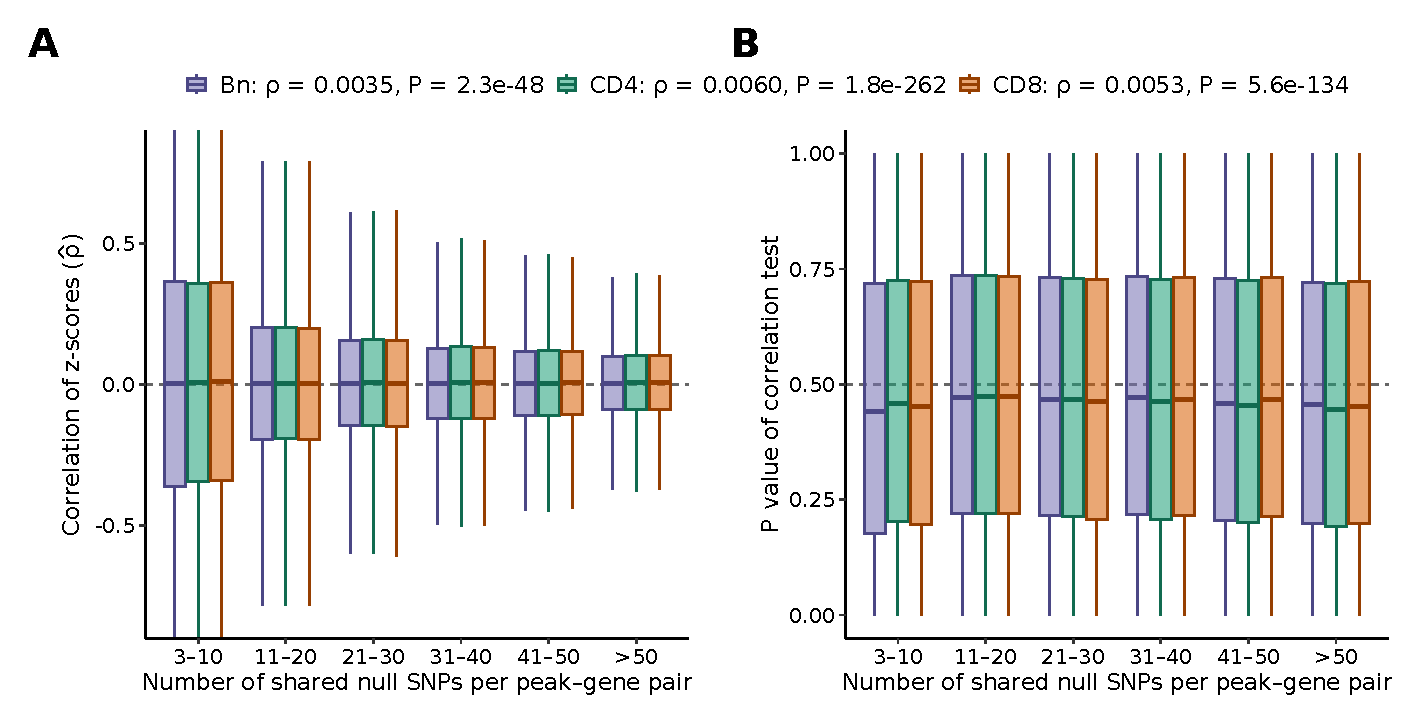
\includegraphics[width=\linewidth]{Figure_S1.pdf}
\caption[Null-SNP diagnostics in Bn, CD4 T cells, and CD8 T cells]{Null-SNP diagnostics in Bn, CD4 T cells, and CD8 T cells.
\textbf{A,} Pair-level correlations of caQTL and eQTL z-scores,
grouped by the number of shared pruned null SNPs; boxes show the three cell
types side by side (Bn, purple; CD4 T cells, green; CD8 T cells, orange). The legend gives the
global correlation \(\rho\) and its p-value for each cell type.
\textbf{B,} Corresponding p-values of the pair-level correlation tests.
The dashed lines mark zero correlation in A and a p-value of 0.5 in B, the
values expected under the null. The analyses included 547,452 (Bn), 1,051,953
(CD4 T cells), and 686,829 (CD8 T cells) peak--gene pairs, based on 17,074,938, 33,263,695, and
21,537,822 SNP--pair observations, respectively.
Global summaries pool SNP--pair observations, so a variant may occur
in multiple pairs. This diagnostic does not itself establish MR calibration.}
\label{fig:supp-qc}
\end{figure}

\begin{figure}[htbp]
\centering
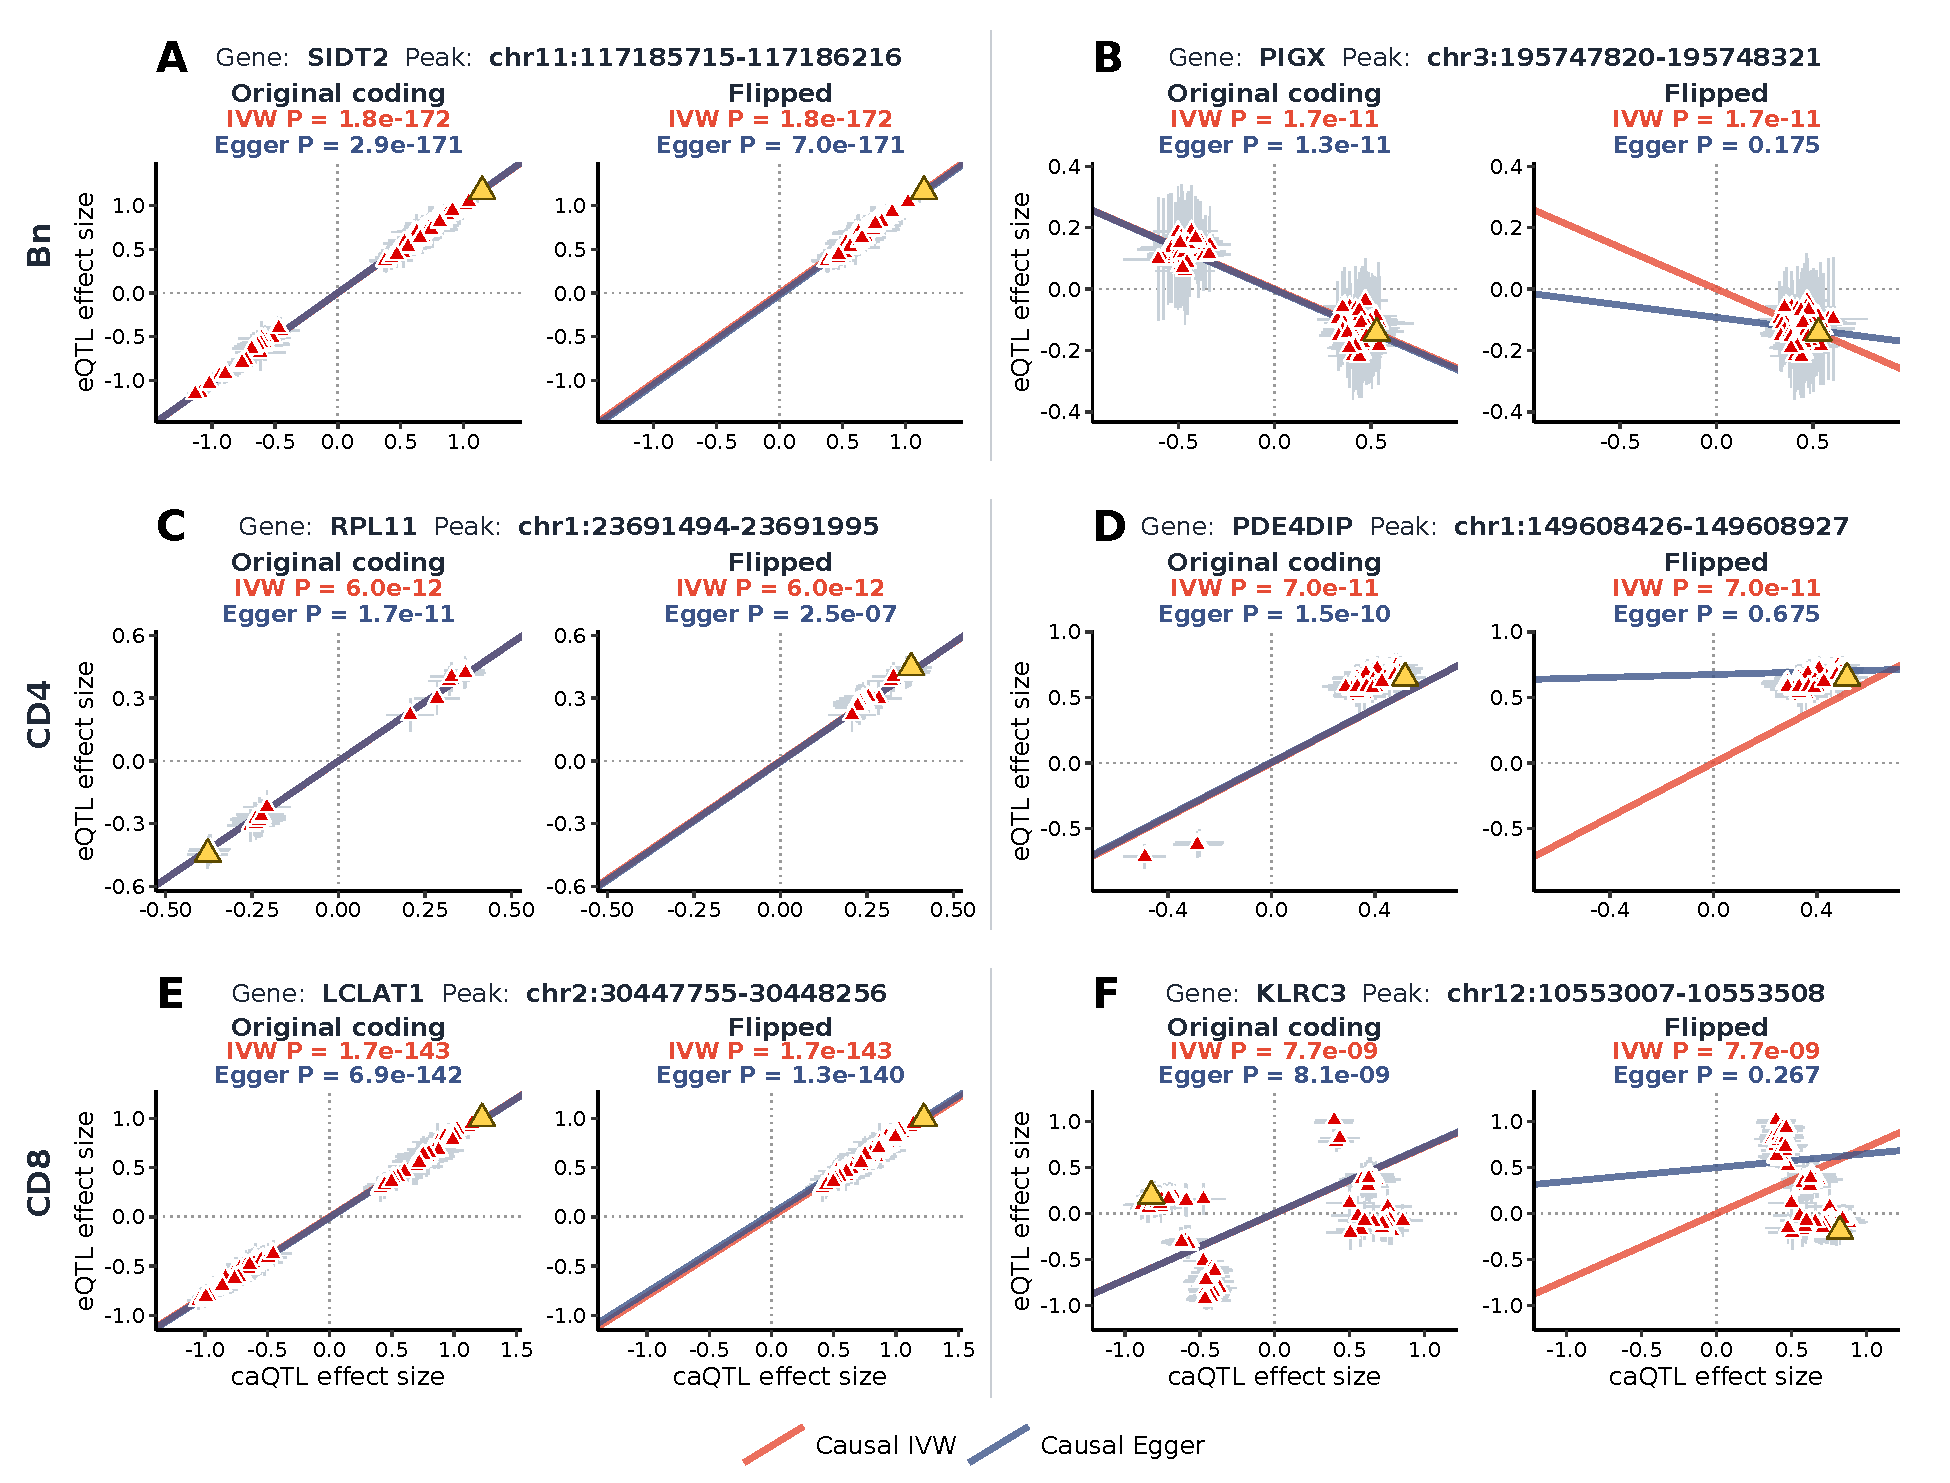
\includegraphics[width=\linewidth]{Figure_S2.pdf}
\caption[MR-Egger estimates with and without allele orientation in Bn, CD4 T cells, and CD8 T cells]{MR-Egger estimates with and without allele orientation in Bn, CD4 T cells, and CD8 T cells.
Rows show Bn, CD4 T cells, and CD8 T cells, and each pair of plots is one
peak--gene pair. \textbf{A,} pairs whose estimates change little with orientation
(SIDT2 in Bn, 194 SNPs; RPL11 in CD4 T cells, 25 SNPs; LCLAT1 in CD8 T cells, 195 SNPs).
\textbf{B,} pairs whose MR-Egger estimate changes markedly (PIGX in Bn, 136 SNPs;
PDE4DIP in CD4 T cells, 74 SNPs; KLRC3 in CD8 T cells, 134 SNPs). For each pair, the
left plot (No flipping) uses the original allele coding and the right plot (Flipping)
orients the pair so that the caQTL effect is positive, as in the MR analysis; both plots
share axis ranges. Red and blue lines are the IVW and MR-Egger fits, and the P values
above each plot are the corresponding IVW and MR-Egger P values. Red triangles are SNPs
and gray bars are 95\% confidence intervals. IVW is unchanged by orientation.}
\label{fig:supp-flip}
\end{figure}

\begin{figure}[htbp]
\centering
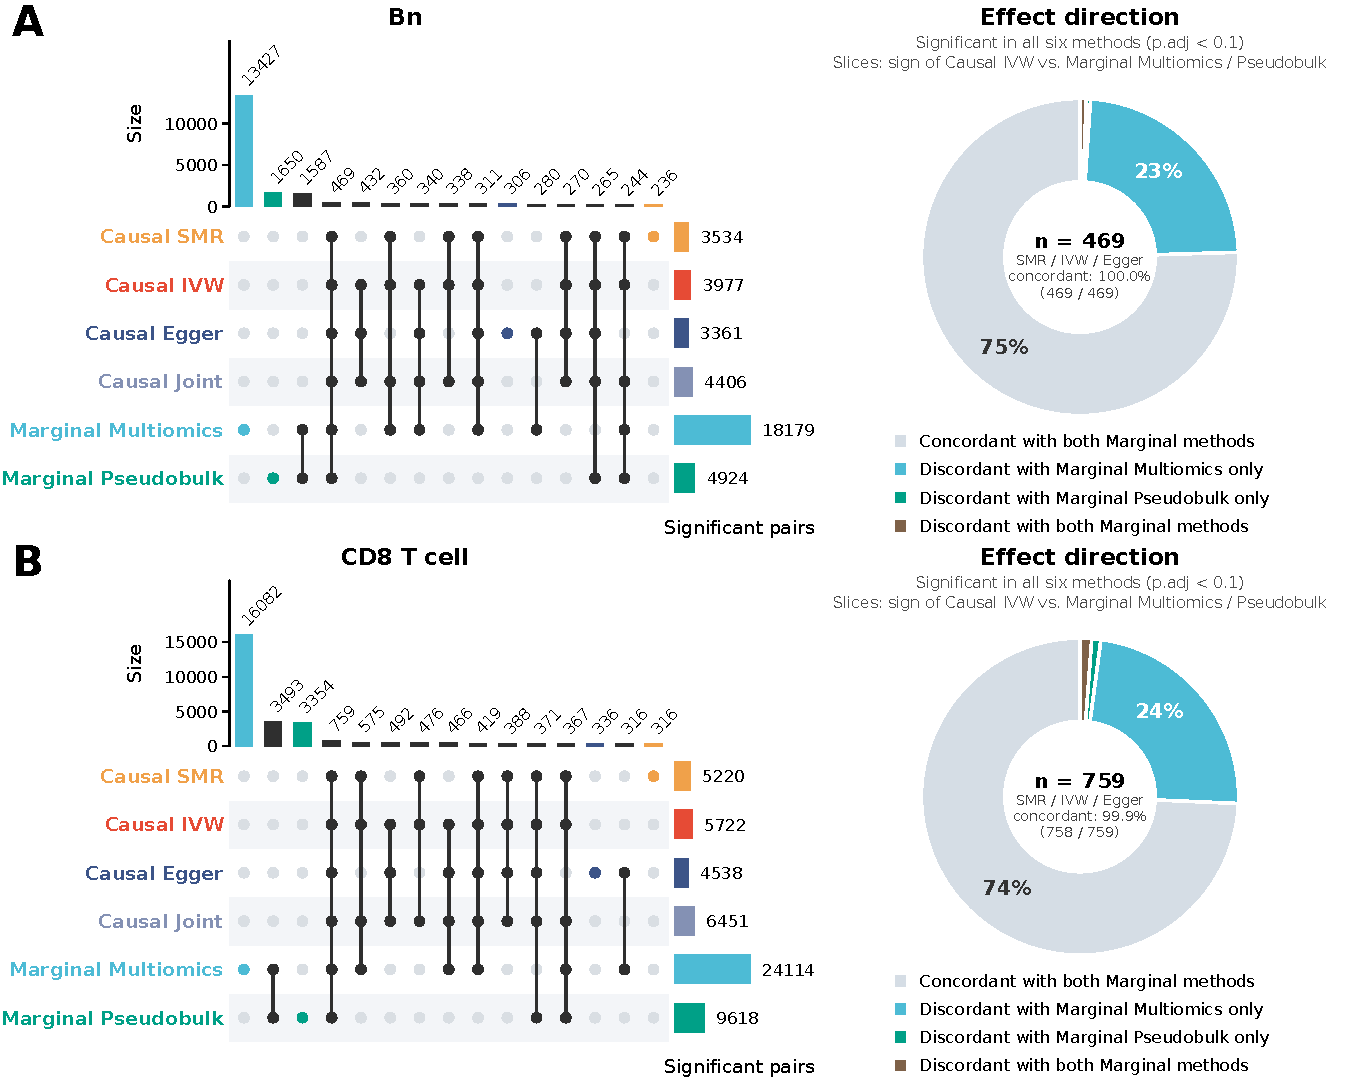
\includegraphics[width=\linewidth]{Figure_S3.pdf}
\caption[Overlap and effect directions of significant links in Bn and CD8 T cells]{Overlap and effect directions of significant links in Bn and CD8 T cells.
\textbf{A,} Bn; \textbf{B,} CD8 T cells. In each row, left: UpSet plot of the 15 largest distinct
significance combinations across six methods at within-gene BH-adjusted \(\q<0.1\); top bars give
the size of each combination, and right bars give the number of significant pairs for each method.
Right: among links significant in all six methods, the sign of the IVW estimate relative to the
signs of the two marginal correlations (categories in the legend below the ring); the center
reports the number of such links and the proportion whose SMR, IVW, and Egger estimates agree in
sign. ``Causal Joint'' denotes CCT. The corresponding CD4 T cell comparison is shown in Fig~1B--C.}
\label{fig:supp-bn-cd8}
\end{figure}

\begin{figure}[htbp]
\centering
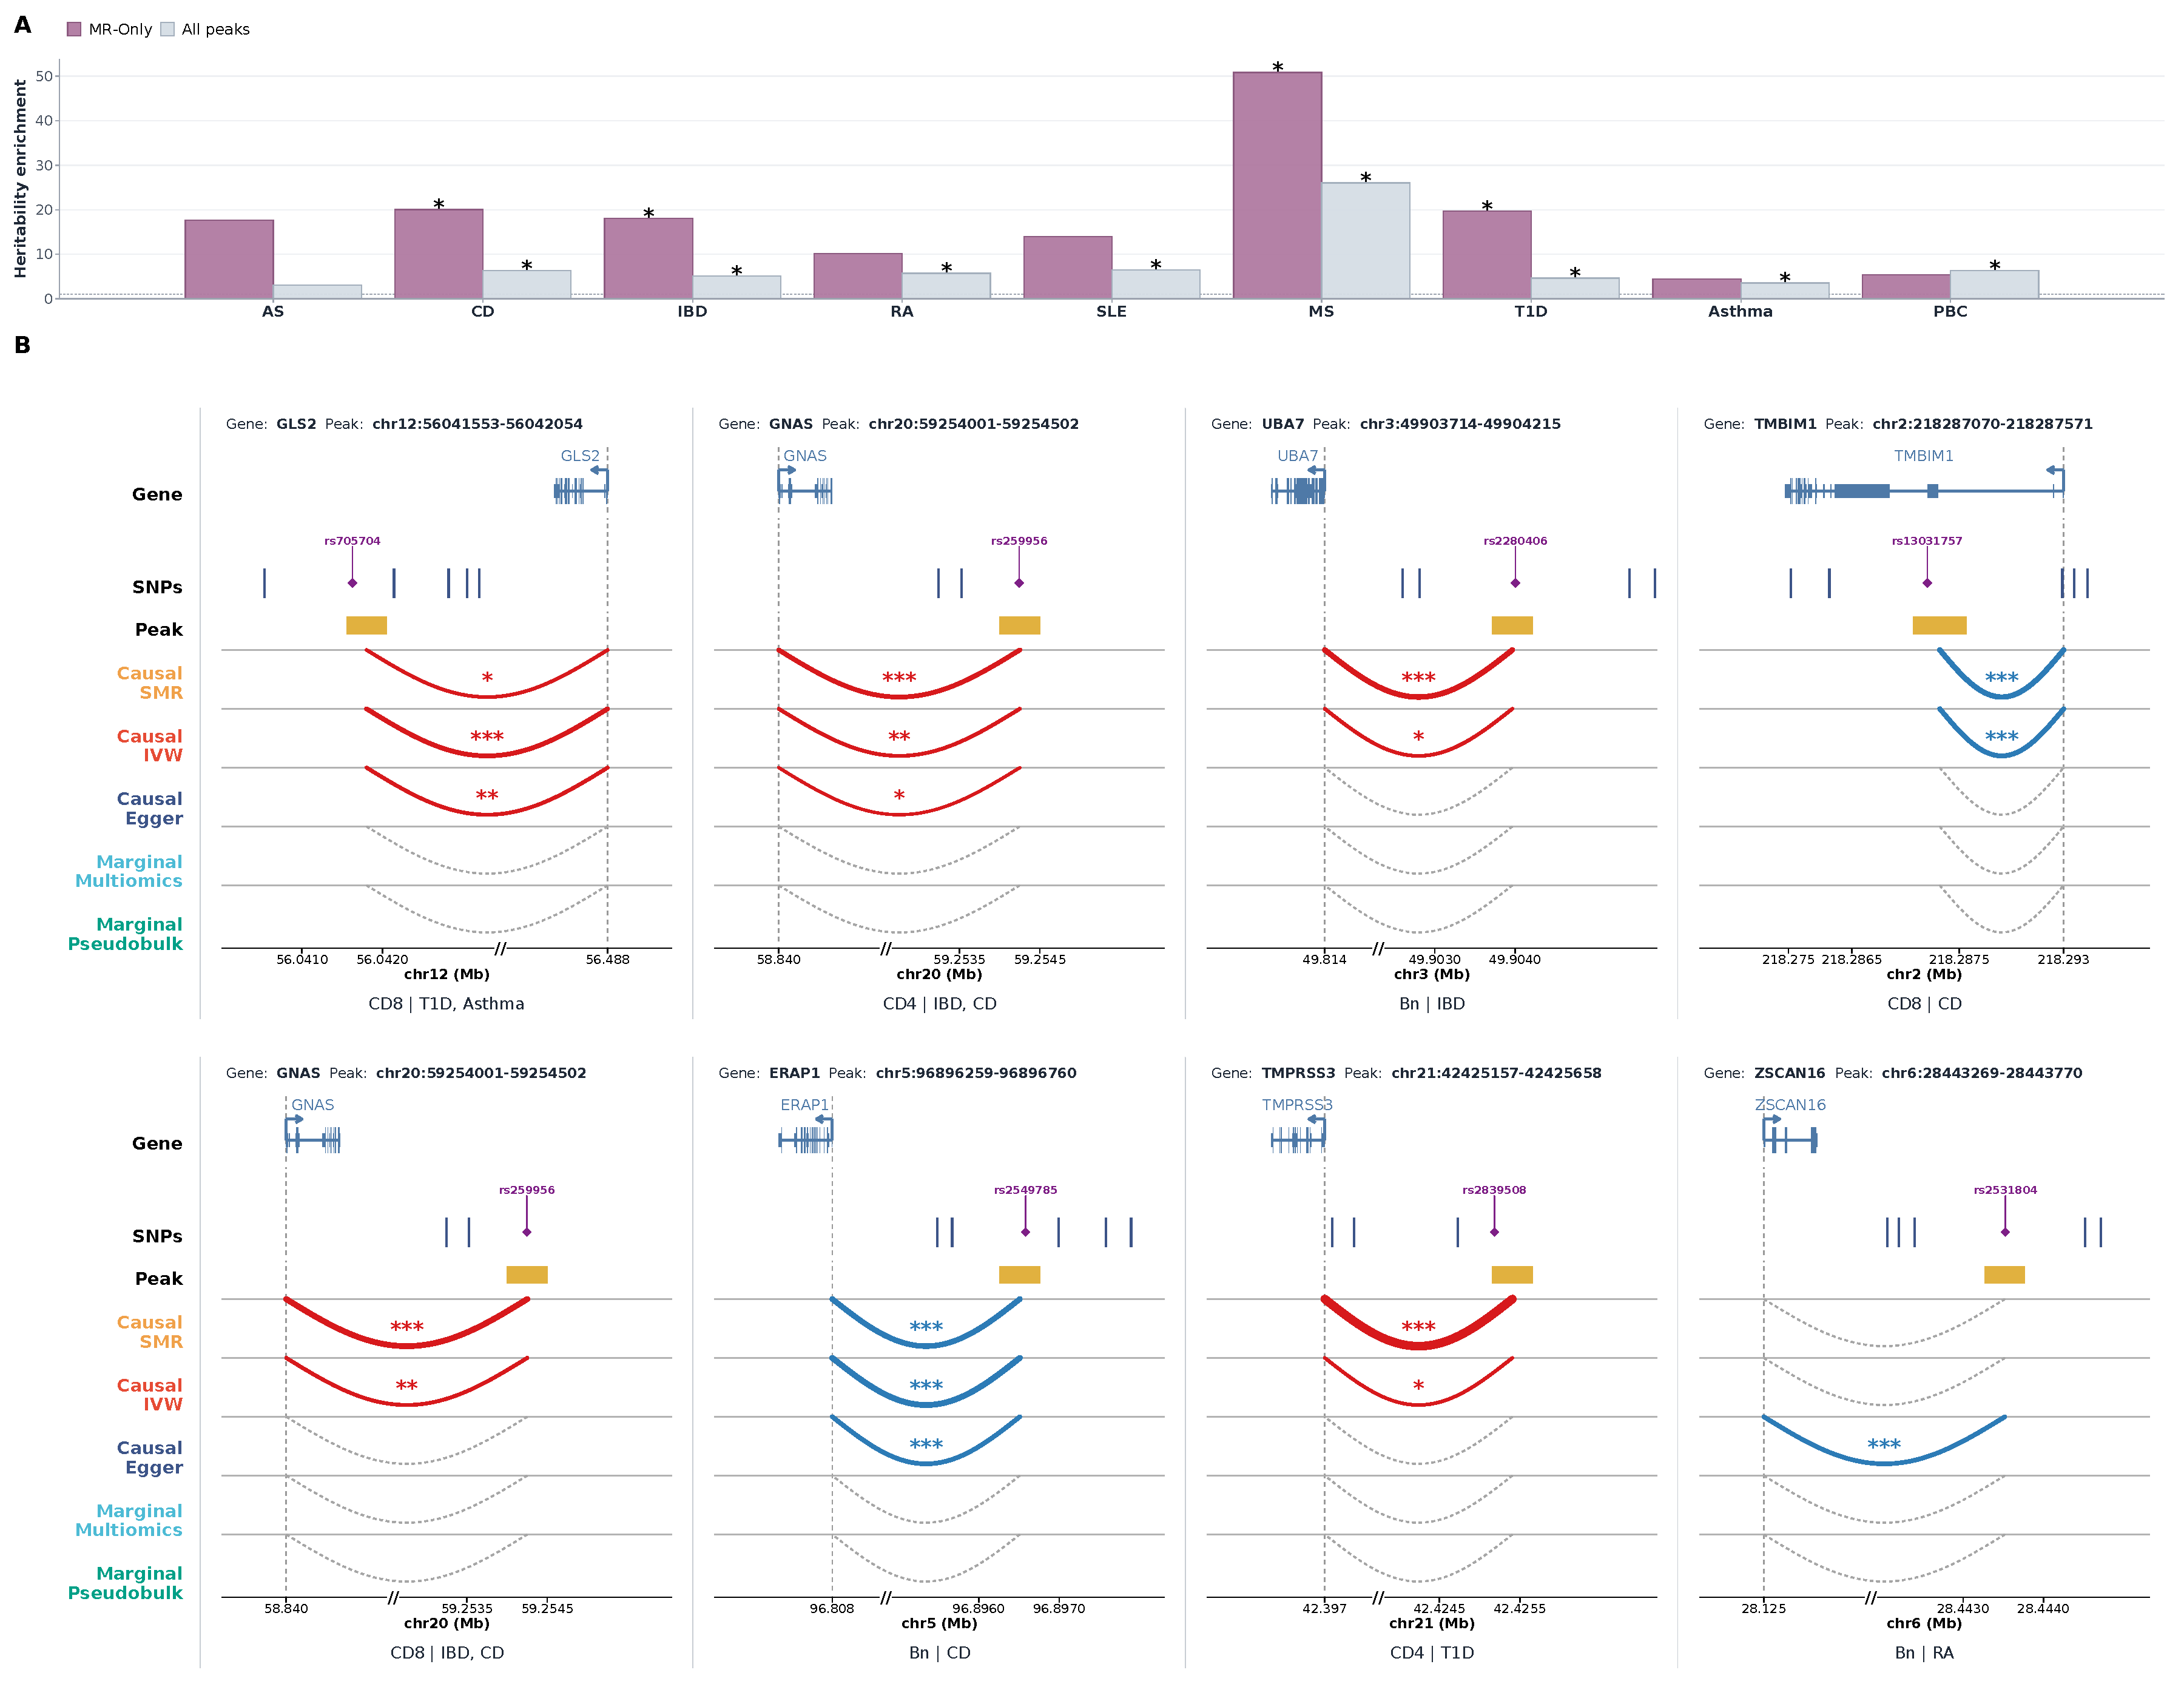
\includegraphics[width=\linewidth]{Figure_S4.pdf}
\caption[Sharing of significant links among Bn, CD4 T cells, and CD8 T cells for each method]{Sharing of significant links among Bn, CD4 T cells, and CD8 T cells for each method.
\textbf{A--F,} causal SMR, causal IVW, causal Egger, causal joint, marginal multiomics, and
marginal pseudobulk. To compare the same pairs across cell types, each diagram is restricted to
the 14,890 candidate peak--gene pairs that were tested in all three cell types (of 40,087,
85,527, and 50,931 pairs tested in Bn, CD4 T cells, and CD8 T cells, respectively). For each
method, the circle of a cell type contains the common pairs with \(\q<0.1\) in that cell type, where
\(\q\) is the within-gene BH-adjusted P value of that cell type's own analysis; pairs were matched
by peak and gene. Numbers inside the diagram give the number of links in each region and, in
parentheses, its percentage of all links significant in at least one cell type for that method.
Labels outside each circle give the number of that cell type's links that fall in the common
pairs over the total number of links of that method in that cell type (all pairs tested in that
cell type), with the percentage in parentheses. Circle areas are not proportional to set sizes.
Marginal multiomics correlations were computed on WNN metacells from an external PBMC dataset
without cell-type separation, so a common pair has the same unadjusted P value in all three
cell types and differs only in the within-gene BH adjustment.}
\label{fig:supp-venn}
\end{figure}

\begin{figure}[htbp]
\centering
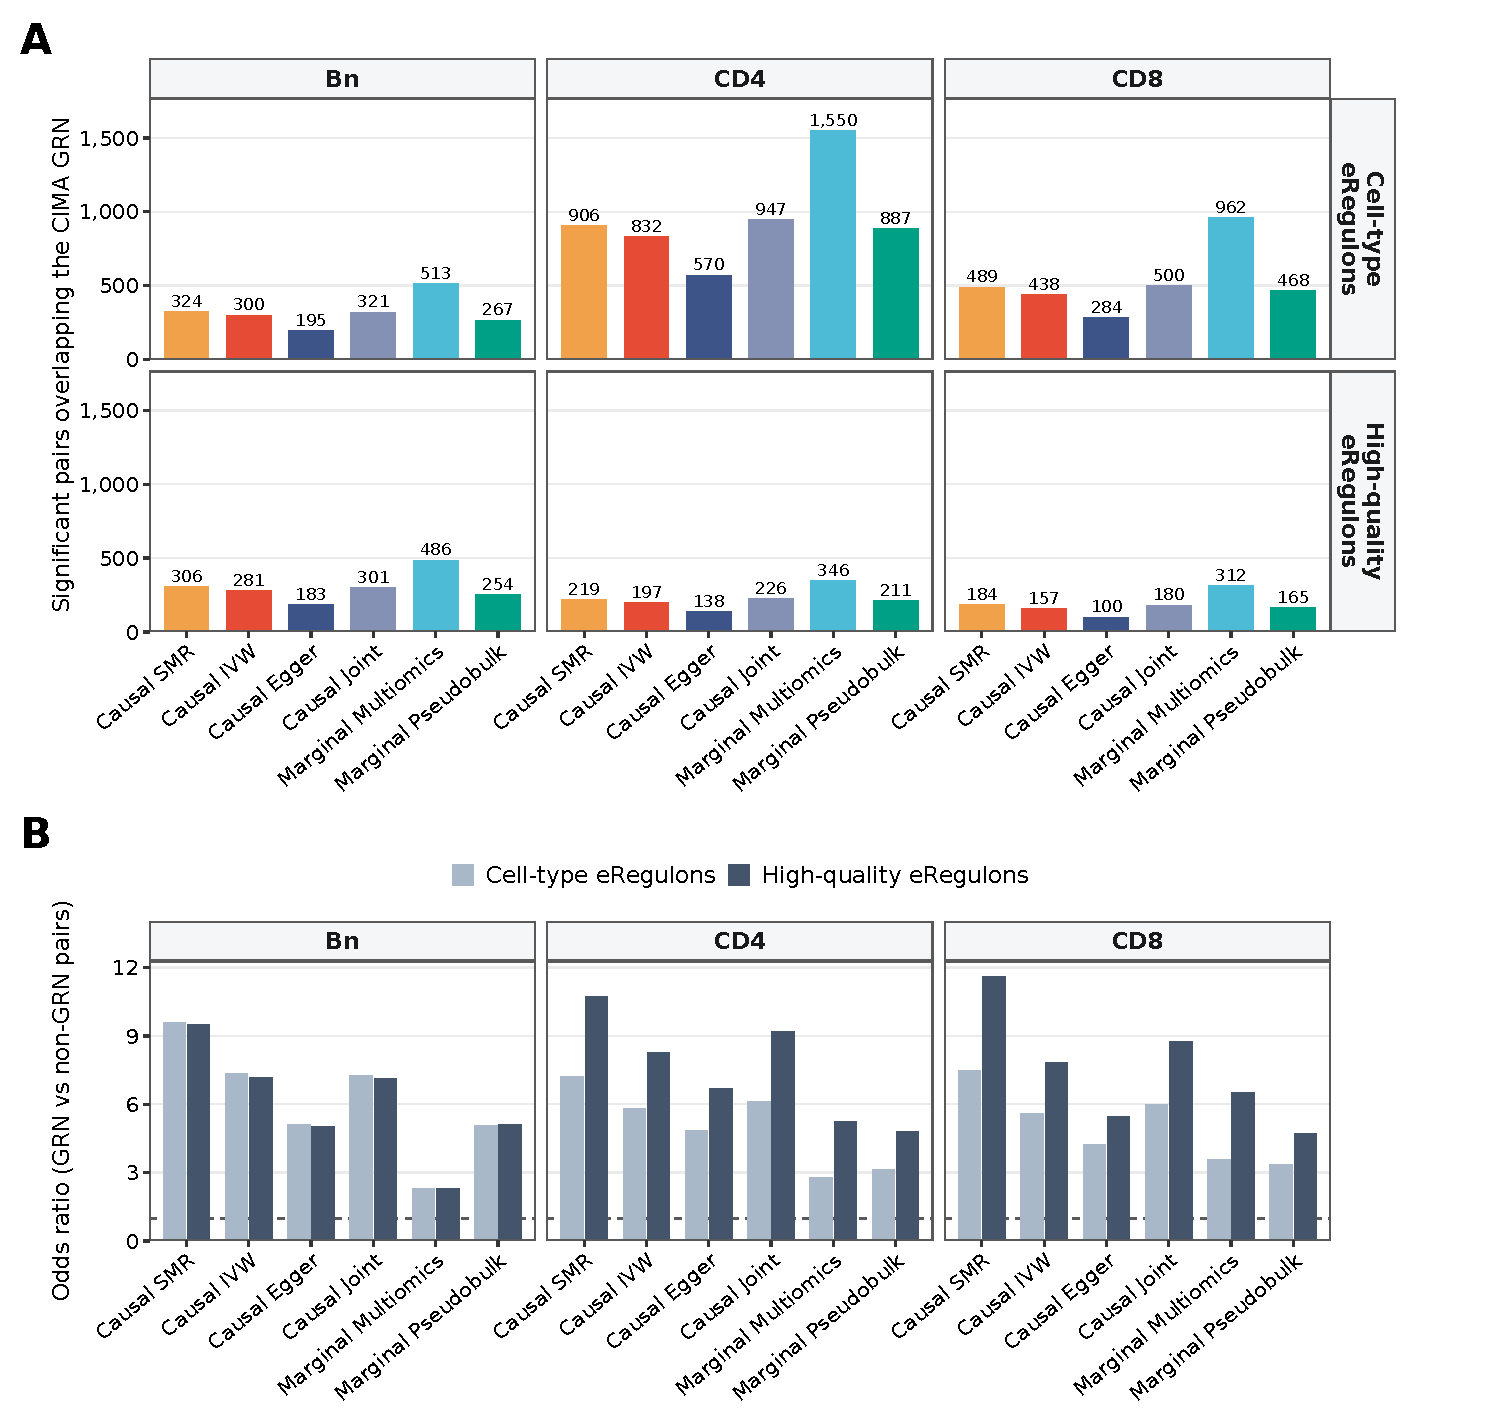
\includegraphics[width=\linewidth]{Figure_S5.pdf}
\caption[Overlap of MR-only links with regulatory references compared with all candidate peaks]{Overlap of MR-only links with regulatory references compared with all candidate peaks.
\textbf{A--F,} GTEx, EnhancerAtlas, FANTOM5, 4DGenome, HiChIP, and PCHi-C (PCHiC in the
figure). MR-only links (\(\q<0.1\) for at least one of causal IVW, causal Egger, and causal SMR,
and \(\q\geq0.1\) for both marginal methods; see Methods) were pooled across the three cell types.
For each gene, \(N\) is the number of candidate peaks (union across cell types), \(K\) the number
of these peaks that overlap the gene's reference regions, \(n_{\mathrm{sig}}\) the number of
peaks of the gene's MR-only links (union across cell types), and \(k\) the number of these
MR-only peaks that overlap the reference regions. For HiChIP and PCHi-C, the reference regions
are the union of the B cell, CD4 T cell, and CD8 T cell interactions. Genes with \(K>0\) and
\(N>K\) were included. The x-axis is the background overlap ratio \(K/N\) and the y-axis the
MR-only overlap ratio \(k/n_{\mathrm{sig}}\); both axes are on a square-root scale. Light green
points are individual genes; genes outside the plotted range are not shown. About 55\% of genes
have a single MR-only peak, so per-gene ratios take few distinct values and form horizontal
bands, including the band at zero. Dark blue points: in each panel, genes were divided into
eight groups of equal size by \(K/N\), and each point gives the pooled ratios \(\sum K/\sum N\)
and \(\sum k/\sum n_{\mathrm{sig}}\) of a group. Error bars are 95\% bootstrap confidence intervals
of \(\sum k/\sum n_{\mathrm{sig}}\) (2,000 resamples of genes within each group, percentile
method). The dashed line is \(y=x\), the overlap expected if MR-only peaks overlapped the
references at the background rate; the shaded area above it marks higher overlap among
MR-only peaks. The lower right of each panel gives the pooled fold enrichment
\((\sum k/\sum n_{\mathrm{sig}})/(\sum K/\sum N)\) and the P value of a hypergeometric test on
the summed counts, computed as in \ref{tab:supp-hyper-p} and \ref{tab:supp-hyper-fold} Tables.
Panel E is also shown as Fig~3D of the main text.}
\label{fig:supp-mronly-ref}
\end{figure}

% S6.1--S6.3 Fig: Figure_S6.pdf has one page per cell type (Bn, CD4 T cells, CD8 T cells).
% The three pages are numbered S6.1, S6.2 and S6.3 Fig: \SixSub sets the number inside each
% figure environment (local), and the figure counter stays at 6 for S6.2 and S6.3.
% All three use the same graphic height; the full legend shared by the three figures is on
% its own page before them, and each caption is short.
\newcommand{\SixSub}[1]{\renewcommand{\thefigure}{S6.#1}\renewcommand{\theHfigure}{supp.6.#1}}
\clearpage
{\small
\noindent\textbf{Legend for S6.1--S6.3 Figs. Pairwise relationships among the five methods
with an effect estimate in Bn, CD4 T cells, and CD8 T cells.}
S6.1, S6.2, and S6.3 Figs show Bn, CD4 T cells, and CD8 T cells, respectively, each using all
candidate peak--gene pairs tested in that cell type (40,087, 85,527, and 50,931 pairs). Causal joint is not shown because it combines
P values and has no effect estimate. \textbf{A,} effect estimates: the MR estimate \(\beta\) for
causal SMR, causal IVW, and causal Egger, and the Spearman correlation coefficient \(\rho\) for
marginal multiomics and marginal pseudobulk. \textbf{B,} signed \(-\log_{10}P\), that is, the sign
of the effect estimate multiplied by \(-\log_{10}P\). In each matrix, the diagonal gives the
method name and the distribution of that method's values across pairs (kernel density; the curve
height is rescaled within the panel, so only its shape is informative). Panels below the diagonal
show the two-dimensional kernel density of pairs, with the method of the column on the x-axis and
the method of the row on the y-axis; color intensity increases with the fourth root of the density
so that low-density regions remain visible. Panels above the diagonal give the Spearman
correlation \(r\) between the two methods across all pairs; text size and background shade
increase with \(r\). Dotted lines mark zero. The dashed line is \(y=x\); in A it is drawn only
between MR methods, whose estimates share units, and in B it is drawn in all panels. Axes are
symmetric around zero and cover the 99th percentile of absolute values across the three cell
types: in A, each method has its own range (\(\pm1.5\) for causal SMR and causal IVW, \(\pm2.5\)
for causal Egger, \(\pm0.75\) for marginal multiomics, and \(\pm0.35\) for marginal pseudobulk);
in B, all methods share \(\pm11\). Pairs outside these ranges (0.3--1.9\% per method and cell
type) are omitted from the density panels but included in \(r\). Marginal multiomics correlations
were computed on WNN metacells from an external PBMC dataset without cell-type separation.\par}
\clearpage

\begin{figure}[p]
\SixSub{1}
\centering
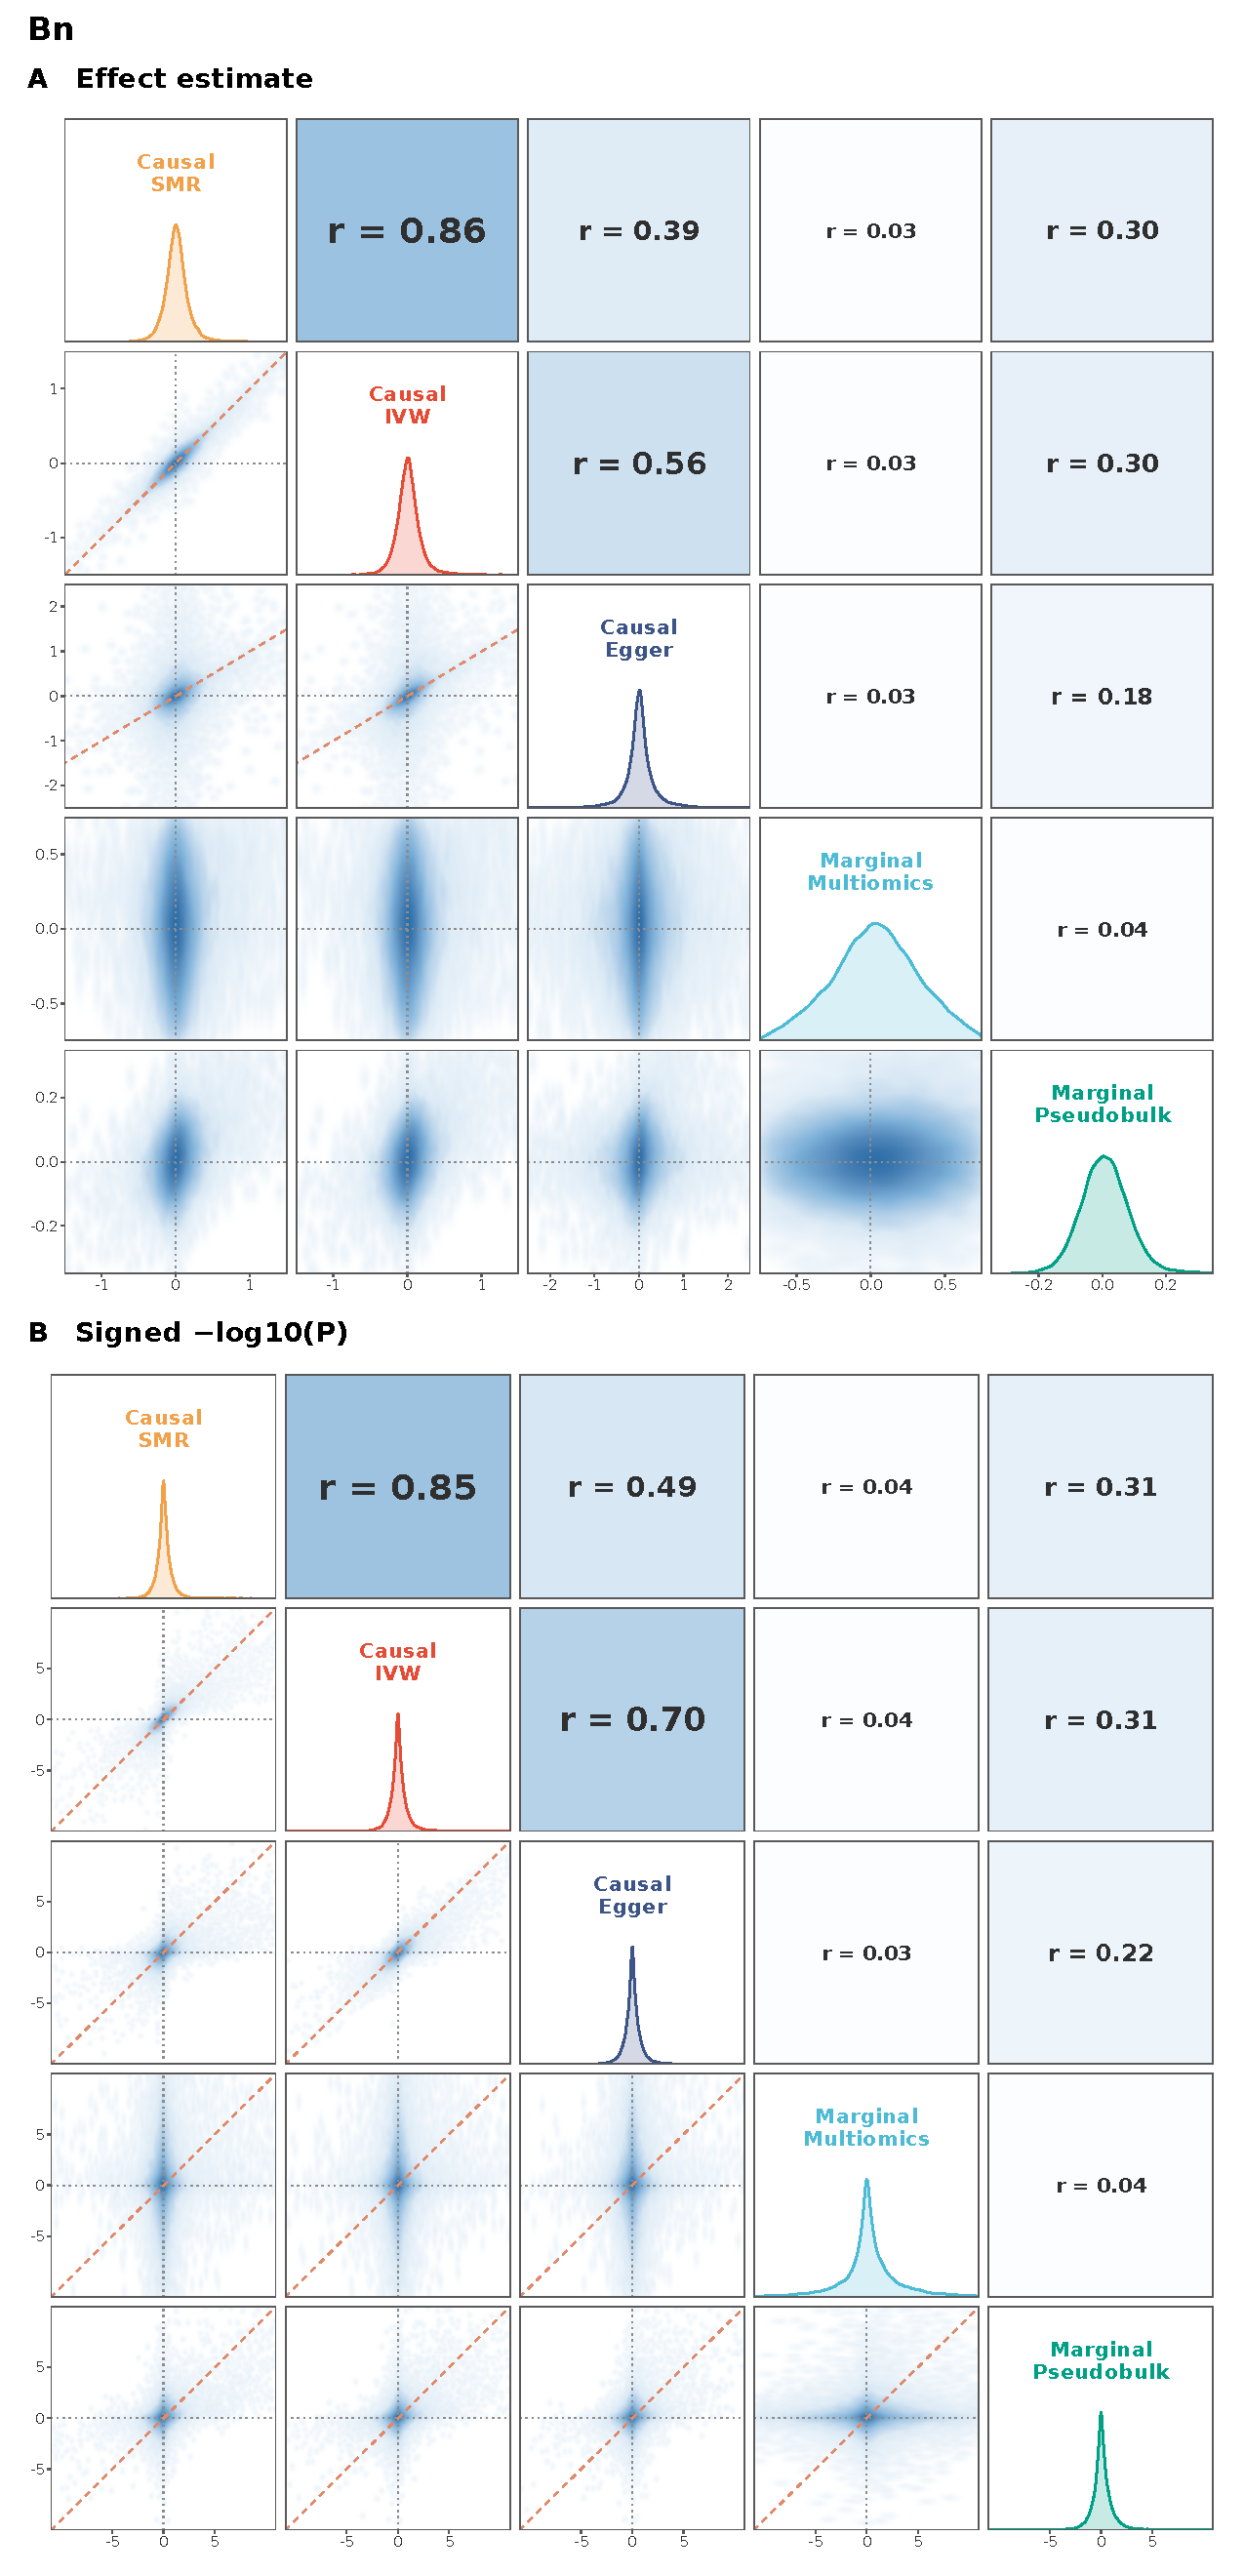
\includegraphics[height=0.86\textheight,page=1]{Figure_S6.pdf}
\caption[Pairwise relationships among the five methods with an effect estimate in Bn]{Pairwise relationships among the five methods with an effect estimate in Bn.
Based on the 40,087 candidate peak--gene pairs tested in Bn. \textbf{A,} effect estimates;
\textbf{B,} signed \(-\log_{10}P\). See the shared legend for S6.1--S6.3 Figs.}
\label{fig:supp-method-cor}
\end{figure}

\begin{figure}[p]
\SixSub{2}\addtocounter{figure}{-1}
\centering
\includegraphics[height=0.86\textheight,page=2]{Figure_S6.pdf}
\caption[Pairwise relationships among the five methods with an effect estimate in CD4 T cells]{Pairwise relationships among the five methods with an effect estimate in CD4 T cells.
Based on the 85,527 candidate peak--gene pairs tested in CD4 T cells. \textbf{A,} effect estimates;
\textbf{B,} signed \(-\log_{10}P\). See the shared legend for S6.1--S6.3 Figs.}
\label{fig:supp-method-cor-cd4}
\end{figure}

\begin{figure}[p]
\SixSub{3}\addtocounter{figure}{-1}
\centering
\includegraphics[height=0.86\textheight,page=3]{Figure_S6.pdf}
\caption[Pairwise relationships among the five methods with an effect estimate in CD8 T cells]{Pairwise relationships among the five methods with an effect estimate in CD8 T cells.
Based on the 50,931 candidate peak--gene pairs tested in CD8 T cells. \textbf{A,} effect estimates;
\textbf{B,} signed \(-\log_{10}P\). See the shared legend for S6.1--S6.3 Figs.}
\label{fig:supp-method-cor-cd8}
\end{figure}
\FloatBarrier % keep S6.1--S6.3 right after their legend page (before the tables)

% S7.1--S7.3 Fig: Figure_S7.pdf has one page per cell type (Bn, CD4 T cells, CD8 T cells);
% numbered like S6.1--S6.3 (\SevenSub is local to each figure; the counter stays at 7).
\newcommand{\SevenSub}[1]{\renewcommand{\thefigure}{S7.#1}\renewcommand{\theHfigure}{supp.7.#1}}
\clearpage
{\small
\noindent\textbf{Legend for S7.1--S7.3 Figs. Genome-wide association signals of the six methods
in Bn, CD4 T cells, and CD8 T cells.}
S7.1, S7.2, and S7.3 Figs show Bn, CD4 T cells, and CD8 T cells, respectively, each using all
candidate peak--gene pairs tested in that cell type (40,087, 85,527, and 50,931 pairs). Each track
is one method (causal SMR, causal IVW, causal Egger, causal joint, marginal multiomics, and
marginal pseudobulk). Each point is a pair placed at the center of its peak along chromosomes 1--22
(hg38); the y-axis gives \(-\log_{10}P\) on a linear scale with a separate range for each track.
The dashed line marks the Bonferroni threshold (0.05 divided by the number of pairs tested in that
cell type); pairs above it are colored orange for causal methods and green for marginal methods,
and the other pairs are shown in alternating shades of gray by chromosome. In each track, up to
eight genes above the threshold are labeled at their strongest pair, with at most one label per
5 Mb on a chromosome. Magenta diamonds mark the example pairs of Fig~2 in the cell type in which
they were shown (\textit{SIDT2} in Bn; \textit{RPL11}, \textit{ERAP2}, and \textit{ARPC1B} in CD4 T
cells), labeled in every track at their actual position whether or not they pass the threshold.
CD8 T cells have no example pair.\par}
\clearpage

\begin{figure}[p]
\SevenSub{1}
\centering
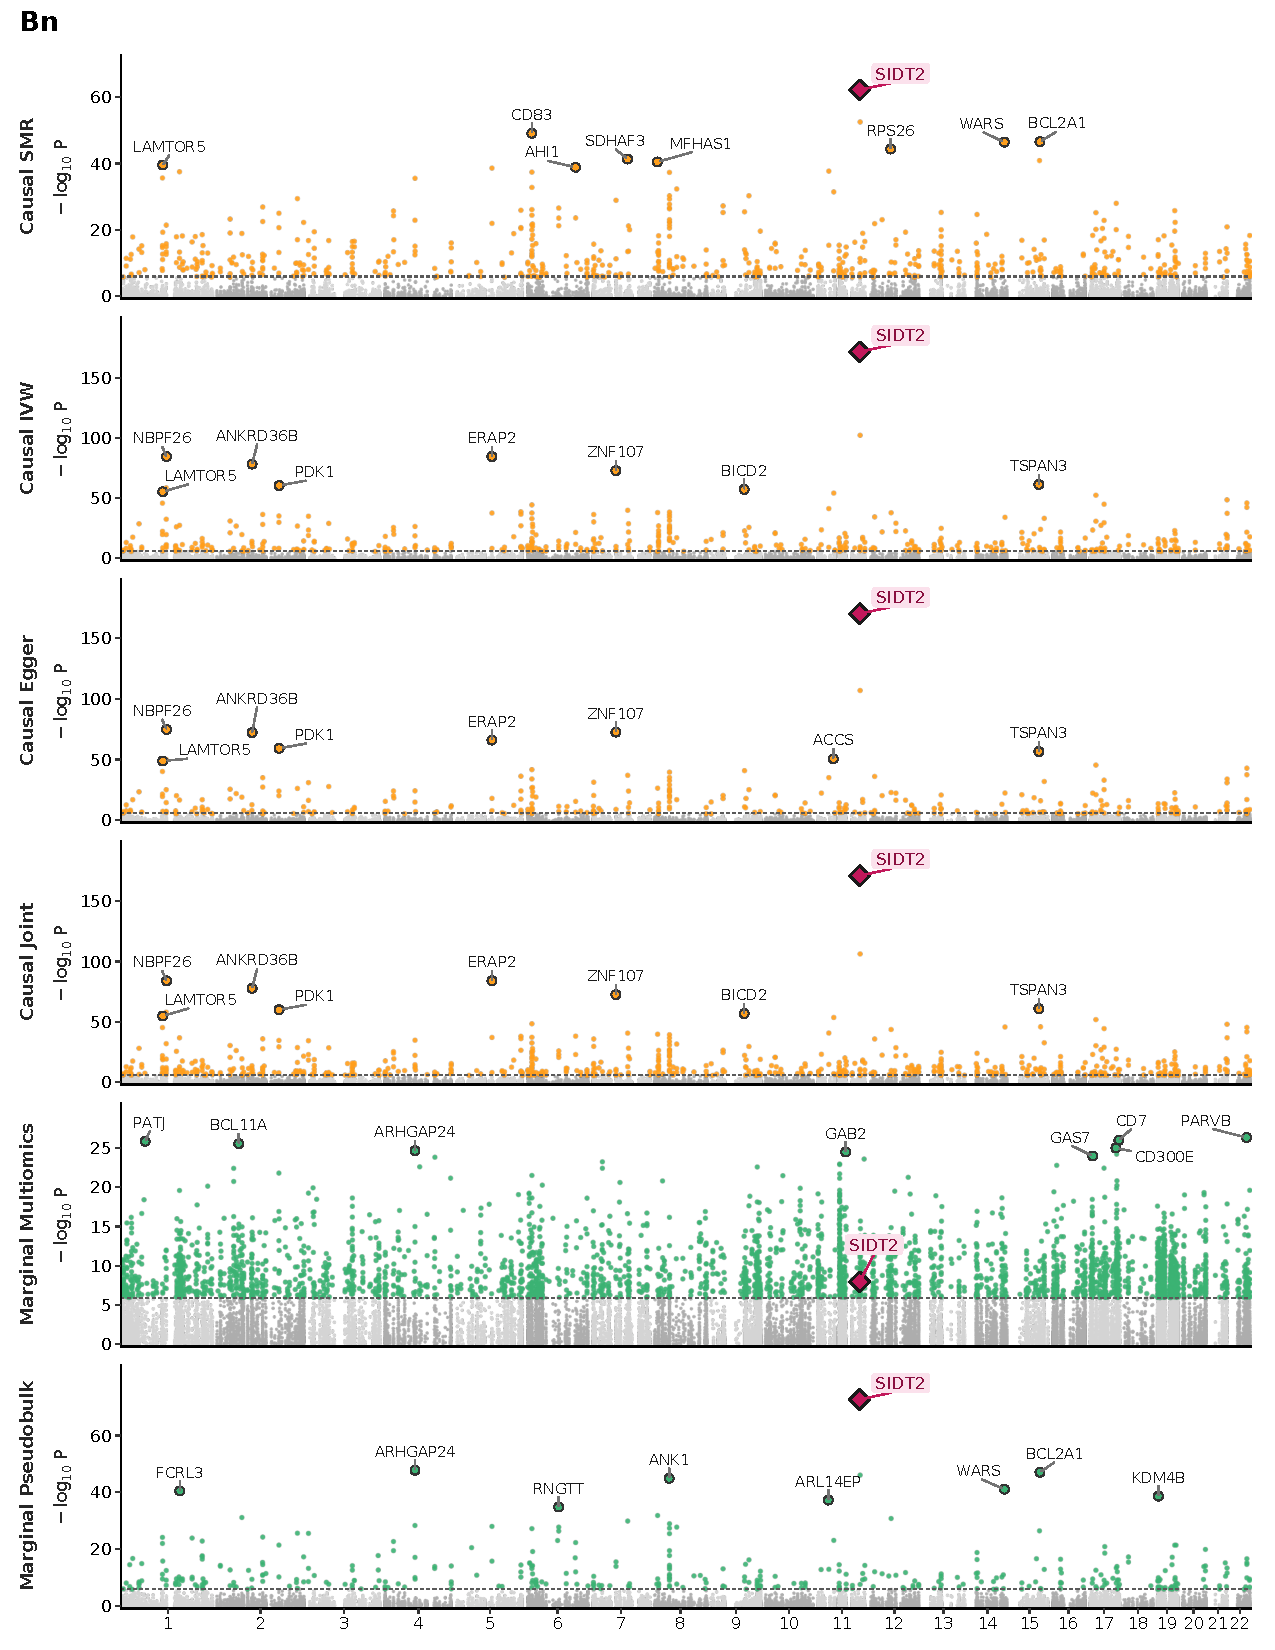
\includegraphics[height=0.86\textheight,page=1]{Figure_S7.pdf}
\caption[Genome-wide association signals of the six methods in Bn]{Genome-wide association signals of the six methods in Bn.
Based on the 40,087 candidate peak--gene pairs tested in Bn. See the shared legend for S7.1--S7.3 Figs.}
\label{fig:supp-manhattan}
\end{figure}

\begin{figure}[p]
\SevenSub{2}\addtocounter{figure}{-1}
\centering
\includegraphics[height=0.86\textheight,page=2]{Figure_S7.pdf}
\caption[Genome-wide association signals of the six methods in CD4 T cells]{Genome-wide association signals of the six methods in CD4 T cells.
Based on the 85,527 candidate peak--gene pairs tested in CD4 T cells. See the shared legend for S7.1--S7.3 Figs.}
\label{fig:supp-manhattan-cd4}
\end{figure}

\begin{figure}[p]
\SevenSub{3}\addtocounter{figure}{-1}
\centering
\includegraphics[height=0.86\textheight,page=3]{Figure_S7.pdf}
\caption[Genome-wide association signals of the six methods in CD8 T cells]{Genome-wide association signals of the six methods in CD8 T cells.
Based on the 50,931 candidate peak--gene pairs tested in CD8 T cells. See the shared legend for S7.1--S7.3 Figs.}
\label{fig:supp-manhattan-cd8}
\end{figure}
\FloatBarrier

\begin{figure}[htbp]
\centering
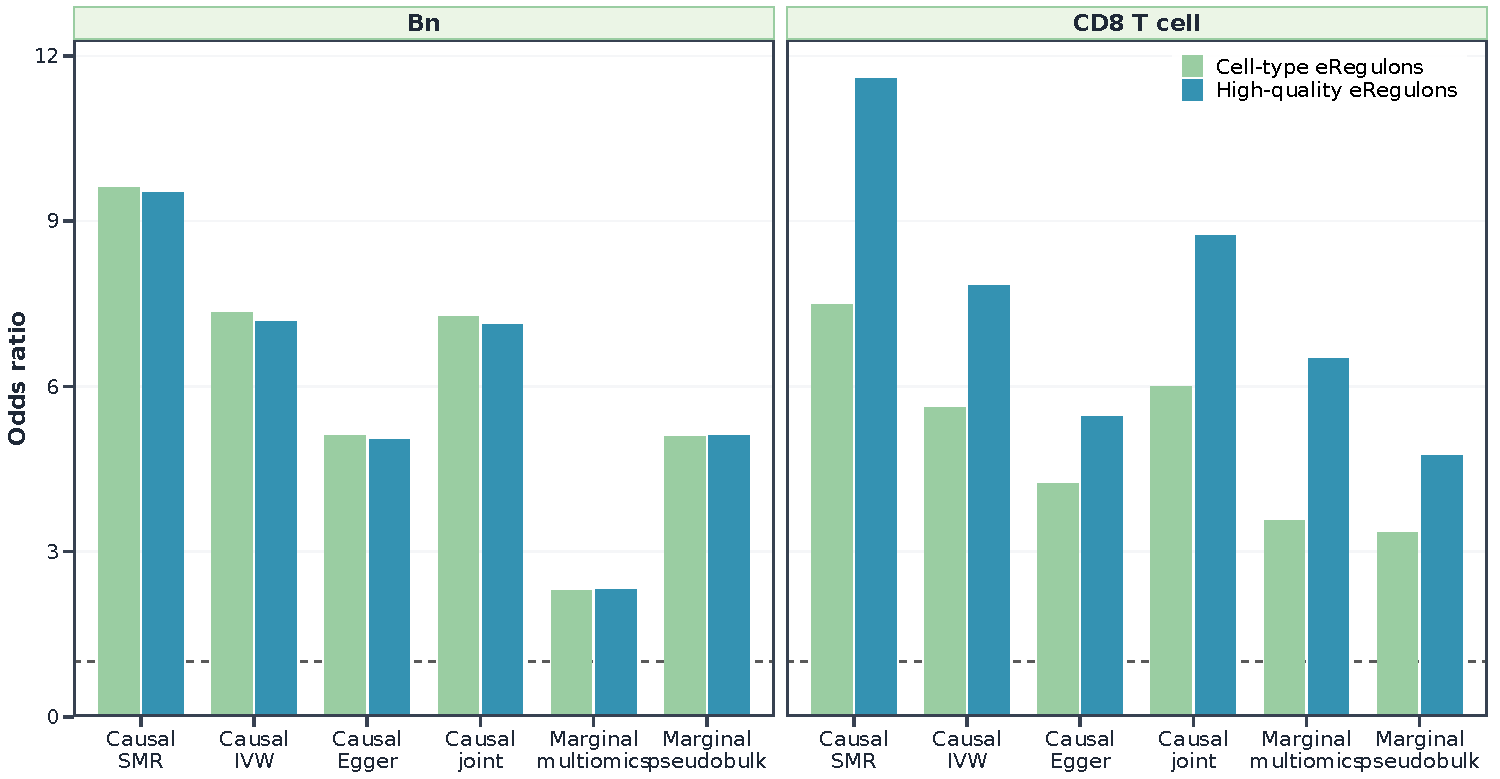
\includegraphics[width=\linewidth]{Figure_S8.pdf}
\caption[Overlap of significant links with the CIMA regulatory network in Bn and CD8 T cells]{Overlap of significant links with the CIMA regulatory network in Bn and CD8 T cells.
Odds ratio for a link significant for each method (within-gene \(\q<0.05\)) being present in the
CIMA SCENIC+ regulatory network, compared with links not in the network (\(2\times2\) table; all
tested pairs in the cell type as background), as in Fig~3E for CD4 T cells. Light bars use
eRegulons active in the cell type (cell-type eRegulons; 864 and 1,364 tested pairs in Bn and CD8
T cells), and dark bars the subset of these that belong to the high-quality eRegulons of the
corresponding lineage (high-quality eRegulons; 817 and 382 tested pairs). Fisher's exact test
\(P<10^{-30}\) for every bar; the dashed line marks an odds ratio of 1.}
\label{fig:supp-grn}
\end{figure}
\FloatBarrier

\begin{table}[htbp]
\centering
\caption{Pooled hypergeometric enrichment p-values across regulatory references.}
\label{tab:supp-hyper-p}
\begingroup
\small
\singlespacing
\setlength{\tabcolsep}{2.5pt}
\renewcommand{\arraystretch}{1.35}
\begin{tabular}{@{}llrrrrrr@{}}
\toprule
Cell type & Method & EnhancerAtlas & FANTOM5 & 4DGenome & GTEx & HiChIP & PCHiC \\
\midrule
Bn & Causal SMR & \(3.7\times10^{-136}\) & \(3.9\times10^{-100}\) & \(2.5\times10^{-58}\) & \(2.3\times10^{-82}\) & \(1.0\times10^{-416}\) & \(3.4\times10^{-58}\) \\
 & Causal IVW & \(1.2\times10^{-108}\) & \(1.5\times10^{-88}\) & \(3.1\times10^{-52}\) & \(1.6\times10^{-71}\) & \(2.7\times10^{-365}\) & \(2.6\times10^{-46}\) \\
 & Causal Egger & \(6.0\times10^{-65}\) & \(8.5\times10^{-68}\) & \(5.6\times10^{-40}\) & \(4.2\times10^{-38}\) & \(9.0\times10^{-286}\) & \(1.1\times10^{-31}\) \\
 & Causal Joint & \(3.7\times10^{-130}\) & \(1.1\times10^{-99}\) & \(2.3\times10^{-54}\) & \(4.2\times10^{-77}\) & \(5.3\times10^{-427}\) & \(9.3\times10^{-57}\) \\
 & Marginal Multiomics & \(6.1\times10^{-138}\) & \(1.3\times10^{-162}\) & \(5.1\times10^{-61}\) & \(2.5\times10^{-61}\) & \(2.1\times10^{-879}\) & \(2.9\times10^{-75}\) \\
 & Marginal Pseudobulk & \(1.6\times10^{-80}\) & \(2.6\times10^{-94}\) & \(2.4\times10^{-44}\) & \(8.4\times10^{-55}\) & \(8.0\times10^{-404}\) & \(4.0\times10^{-54}\) \\
\midrule
CD4 & Causal SMR & \(3.5\times10^{-302}\) & \(6.5\times10^{-107}\) & \(9.4\times10^{-50}\) & \(2.6\times10^{-209}\) & \(1.3\times10^{-911}\) & \(2.0\times10^{-140}\) \\
 & Causal IVW & \(1.2\times10^{-221}\) & \(3.0\times10^{-94}\) & \(3.2\times10^{-47}\) & \(3.6\times10^{-151}\) & \(5.0\times10^{-890}\) & \(2.2\times10^{-154}\) \\
 & Causal Egger & \(2.1\times10^{-109}\) & \(4.9\times10^{-47}\) & \(5.7\times10^{-33}\) & \(9.2\times10^{-98}\) & \(3.0\times10^{-584}\) & \(1.9\times10^{-92}\) \\
 & Causal Joint & \(6.0\times10^{-249}\) & \(6.2\times10^{-109}\) & \(1.1\times10^{-55}\) & \(8.2\times10^{-195}\) & \(4.7\times10^{-981}\) & \(5.6\times10^{-160}\) \\
 & Marginal Multiomics & \(1.7\times10^{-200}\) & \(3.2\times10^{-123}\) & \(6.1\times10^{-40}\) & \(2.3\times10^{-114}\) & \(6.2\times10^{-1875}\) & \(1.3\times10^{-191}\) \\
 & Marginal Pseudobulk & \(1.3\times10^{-137}\) & \(4.7\times10^{-92}\) & \(4.1\times10^{-37}\) & \(5.3\times10^{-97}\) & \(1.6\times10^{-1172}\) & \(1.4\times10^{-158}\) \\
\midrule
CD8 & Causal SMR & \(2.1\times10^{-204}\) & \(1.8\times10^{-72}\) & \(2.4\times10^{-38}\) & \(1.7\times10^{-104}\) & \(1.6\times10^{-614}\) & \(8.6\times10^{-103}\) \\
 & Causal IVW & \(3.1\times10^{-156}\) & \(1.5\times10^{-60}\) & \(1.7\times10^{-34}\) & \(8.7\times10^{-100}\) & \(1.1\times10^{-616}\) & \(6.9\times10^{-83}\) \\
 & Causal Egger & \(3.4\times10^{-104}\) & \(3.1\times10^{-38}\) & \(1.2\times10^{-28}\) & \(6.4\times10^{-55}\) & \(1.2\times10^{-446}\) & \(7.1\times10^{-48}\) \\
 & Causal Joint & \(8.8\times10^{-189}\) & \(1.4\times10^{-76}\) & \(3.9\times10^{-41}\) & \(1.5\times10^{-119}\) & \(4.6\times10^{-687}\) & \(4.2\times10^{-95}\) \\
 & Marginal Multiomics & \(1.7\times10^{-150}\) & \(3.1\times10^{-111}\) & \(2.1\times10^{-34}\) & \(2.9\times10^{-75}\) & \(7.4\times10^{-1466}\) & \(4.1\times10^{-130}\) \\
 & Marginal Pseudobulk & \(1.6\times10^{-104}\) & \(1.4\times10^{-77}\) & \(3.6\times10^{-17}\) & \(9.5\times10^{-57}\) & \(1.0\times10^{-824}\) & \(1.7\times10^{-77}\) \\
\bottomrule
\end{tabular}
\par\medskip
\begin{minipage}{\linewidth}
\footnotesize
For each cell type, method, and reference, an upper-tail hypergeometric
test was applied to counts pooled over eligible genes. For each gene,
\(N\) is the number of background candidate peaks, \(K\) the number
overlapping the reference, \(n_{\mathrm{sig}}\) the number of selected
significant peaks, and \(k\) the selected peaks overlapping the reference.
Eligibility requires \(N>0\), \(K>0\), \(n_{\mathrm{sig}}>0\), and \(N>K\).
The test uses \(\sum N,\sum K,\sum n_{\mathrm{sig}},\sum k\).
Entries are hypergeometric p-values, with no additional adjustment
across the displayed comparisons specified by the source workbook.
Bn, naive B cells; CD4/CD8, naive CD4/CD8 T cells.
Causal Joint is the Cauchy combination (CCT) of SMR, IVW, and MR-Egger;
Marginal Multiomics denotes the WNN metacell correlation and Marginal Pseudobulk
the individual-level pseudobulk correlation.
\end{minipage}
\endgroup
\end{table}

\begin{table}[htbp]
\centering
\caption{Pooled regulatory-reference fold enrichment across cell types and methods.}
\label{tab:supp-hyper-fold}
\begingroup
\small
\singlespacing
\setlength{\tabcolsep}{2.5pt}
\renewcommand{\arraystretch}{1.35}
\begin{tabular}{@{}llrrrrrr@{}}
\toprule
Cell type & Method & EnhancerAtlas & FANTOM5 & 4DGenome & GTEx & HiChIP & PCHiC \\
\midrule
Bn & Causal SMR & \textbf{3.59} & \textbf{6.18} & \textbf{5.00} & \textbf{2.96} & \textbf{4.46} & \textbf{2.70} \\
 & Causal IVW & 3.10 & 5.65 & 4.54 & 2.71 & 4.02 & 2.46 \\
 & Causal Egger & 2.69 & 5.59 & 4.39 & 2.34 & 3.89 & 2.32 \\
 & Causal Joint & 3.20 & 5.67 & 4.42 & 2.70 & 4.12 & 2.56 \\
 & Marginal Multiomics & 1.98 & 3.56 & 2.61 & 1.70 & 3.08 & 1.84 \\
 & Marginal Pseudobulk & 2.49 & 5.03 & 3.76 & 2.34 & 3.76 & 2.38 \\
\midrule
CD4 & Causal SMR & \textbf{3.56} & \textbf{4.45} & \textbf{3.30} & \textbf{3.01} & \textbf{4.65} & 2.55 \\
 & Causal IVW & 2.98 & 4.08 & 3.12 & 2.63 & 4.41 & \textbf{2.61} \\
 & Causal Egger & 2.52 & 3.46 & 3.02 & 2.51 & 4.17 & 2.41 \\
 & Causal Joint & 2.99 & 4.17 & 3.20 & 2.77 & 4.40 & 2.56 \\
 & Marginal Multiomics & 1.84 & 2.49 & 1.85 & 1.68 & 3.35 & 1.85 \\
 & Marginal Pseudobulk & 2.05 & 3.10 & 2.30 & 1.94 & 3.78 & 2.16 \\
\midrule
CD8 & Causal SMR & \textbf{3.65} & \textbf{4.64} & \textbf{3.60} & \textbf{2.76} & \textbf{5.46} & \textbf{2.70} \\
 & Causal IVW & 3.13 & 4.19 & 3.36 & 2.69 & 5.26 & 2.52 \\
 & Causal Egger & 2.90 & 3.84 & 3.48 & 2.40 & 5.08 & 2.29 \\
 & Causal Joint & 3.21 & 4.41 & 3.46 & 2.75 & 5.22 & 2.53 \\
 & Marginal Multiomics & 1.90 & 2.81 & 2.00 & 1.68 & 4.01 & 1.88 \\
 & Marginal Pseudobulk & 2.21 & 3.60 & 2.11 & 1.96 & 4.62 & 2.07 \\
\bottomrule
\end{tabular}
\par\medskip
\begin{minipage}{\linewidth}
\footnotesize
Fold enrichment is \((\sum k/\sum n_{\mathrm{sig}})/(\sum K/\sum N)\),
using the eligible-gene counts defined in \ref{tab:supp-hyper-p} Table.
Values are rounded to two decimal places. Bold indicates the greatest
unrounded enrichment within each cell type and reference column.
Contributing genes and selected-set sizes can differ across methods;
these descriptive values are not paired tests of method superiority.
Bn, naive B cells; CD4/CD8, naive CD4/CD8 T cells.
Causal Joint is the Cauchy combination (CCT) of SMR, IVW, and MR-Egger;
Marginal Multiomics denotes the WNN metacell correlation and Marginal Pseudobulk
the individual-level pseudobulk correlation.
\end{minipage}
\endgroup
\end{table}

\clearpage
\begin{table}[htbp]
\centering
\caption{Data overview for the three cell types analyzed.}
\label{tab:supp-data}
\begingroup
\small
\singlespacing
\setlength{\tabcolsep}{4pt}
\renewcommand{\arraystretch}{1.3}
\begin{tabular}{@{}>{\raggedright\arraybackslash}p{3.3in}rrr@{}}
\toprule
 & Bn & CD4 T cell & CD8 T cell \\
\midrule
\rowcolor{gray!14}\multicolumn{4}{@{}l}{\textbf{Single-cell data used for the pseudobulk correlation (after quality control)}} \\
Individuals (passing RNA and ATAC cell-count filters) & 335 & 372 & 346 \\
scRNA-seq cells & 160,577 & 916,643 & 460,439 \\
scATAC-seq cells & 123,580 & 360,343 & 210,077 \\
scRNA-seq cells per individual, median (IQR) & 436 (315--619) & 2,336 (1,655--3,150) & 1,200 (763--1,760) \\
scATAC-seq cells per individual, median (IQR) & 348 (236--464) & 898 (618--1,278) & 510 (320--845) \\
Genes in the pseudobulk RNA matrix & 36,326 & 36,326 & 36,326 \\
Peaks in the pseudobulk ATAC matrix & 338,036 & 338,036 & 338,036 \\
\rowcolor{gray!14}\multicolumn{4}{@{}l}{\textbf{cis-QTL summary statistics}} \\
eQTL sample size & 405 & 406 & 405 \\
caQTL sample size & 385 & 385 & 384 \\
Peaks with at least one caQTL at \(P<10^{-8}\) & 3,449 & 6,110 & 3,847 \\
\rowcolor{gray!14}\multicolumn{4}{@{}l}{\textbf{Candidate peak--gene pairs and the Mendelian randomization analysis set}} \\
Candidate gene--peak pairs (All\_GenePeak, TSS--peak distance \(<1\)~Mb) & 3,814,826 & 5,146,441 & 4,505,251 \\
With caQTL and eQTL variants in common (at least 3 shared variants) & 46,190 & 109,961 & 62,136 \\
Gene and peak present in both pseudobulk and WNN data & 40,389 & 86,204 & 51,649 \\
After removing pairs with a missing p-value in any base method & 40,153 & 85,782 & 51,123 \\
Final analysis set (IVW residual variance \(\le\) 10) & 40,087 & 85,527 & 50,931 \\
Genes / peaks in the final analysis set & 8,149 / 2,951 & 10,701 / 5,338 & 9,427 / 3,327 \\
Variants (instruments) per pair in the IVW fit, median (IQR) & 22 (10--40) & 22 (10--43) & 22 (9--41) \\
\rowcolor{gray!14}\multicolumn{4}{@{}l}{\textbf{Samples for the marginal correlation methods}} \\
Pseudobulk correlation: individuals & 335 & 372 & 346 \\
WNN correlation: metacells (external PBMC multiome) & 80 & 80 & 80 \\
\bottomrule
\end{tabular}
\par\medskip
\begin{minipage}{\linewidth}
\footnotesize
Bn, naive B cells (CIMA L4 type Bn\_TCL1A); CD4 T cell, naive CD4\(^+\) T cells (CD4\_Tn\_CCR7);
CD8 T cell, naive CD8\(^+\) T cells (CD8\_Tn\_CCR7). The Chinese Immune Multi-Omics Atlas (CIMA;
Yin et al., Science 2026; OMIX009786) comprises scRNA-seq and scATAC-seq data from
428 Chinese adults annotated into 73 L4 immune cell types. The cis-QTL were mapped within
1~Mb of the gene transcription start site or the peak midpoint, using genotypes of the
whole cohort (5,051,397 variants with minor allele frequency \(>0.1\)); the numbers
in the table are specific to the three cell types analyzed here.
Three sample definitions are used: the QTL sample sizes (summary statistics used by the
Mendelian randomization methods), the individuals in the pseudobulk matrices (those passing the
RNA and ATAC cell-count filters; pseudobulk correlation), and 80 metacells of an external PBMC
multiome data set (WNN correlation). The caQTL and eQTL data come from the same cohort, so
the two QTL data sets overlap in samples.
Peaks with at least one caQTL at \(P<10^{-8}\) are counted from the significant caQTL
files used to select instruments; this is a nominal threshold, not the false-discovery-rate-defined
caPeak count of CIMA.
Candidate pairs are All\_GenePeak pairs with at least 3 variants shared between the clumped
caQTL and the eQTL data, whose gene and peak are present in both the pseudobulk and WNN data.
Pairs with a missing p-value in any base method (IVW, MR-Egger, SMR, WNN, pseudobulk) or with
an IVW residual variance above 10 were removed. IQR, interquartile range.
\end{minipage}
\endgroup
\end{table}


\clearpage
\begin{table}[htbp]
\centering
\caption{GWAS used in the S-LDSC analysis (Fig~4A) and in the GWAS-overlap tracks (Fig~4B).}
\label{tab:supp-gwas}
\begingroup
\footnotesize
\singlespacing
\setlength{\tabcolsep}{3pt}
\renewcommand{\arraystretch}{1.35}
\begin{tabular}{@{}>{\raggedright\arraybackslash}p{1.45in}>{\raggedright\arraybackslash}p{1.75in}>{\raggedright\arraybackslash}p{1.35in}r>{\raggedright\arraybackslash}p{0.8in}@{}}
\toprule
Trait & Study or data source & N & SNPs & \(h^2\) (SE) \\
\midrule
Ankylosing spondylitis (AS) & Pan-UK Biobank (\url{https://pan.ukbb.broadinstitute.org/}) & 420,473\newline (1,185 cases / 419,288 controls) & 1,188,036 & 0.0052\newline (0.0017) \\
Crohn's disease (CD) & International IBD Genetics Consortium (\url{https://www.ibdgenetics.org/}) & 367,592\newline (20,873 cases / 346,719 controls) & 1,188,159 & 0.0649\newline (0.0058) \\
Inflammatory bowel disease (IBD) & de Lange et al.~\cite{delange2017ibd} & 59,957 & 1,150,510 & 0.3202\newline (0.0243) \\
Rheumatoid arthritis (RA) & Saevarsdottir et al.~\cite{saevarsdottir2022ra} & 1,026,690 & 1,184,671 & 0.0132\newline (0.0011) \\
Systemic lupus erythematosus (SLE) & Bentham et al.~\cite{bentham2015sle} & 14,267 & 1,163,805 & 0.4567\newline (0.0957) \\
Multiple sclerosis (MS) & International Multiple Sclerosis Genetics Consortium~\cite{sawcer2011ms} & 27,148 & 450,159 & 0.0800\newline (0.0373) \\
Type 1 diabetes (T1D) & Chiou et al.~\cite{chiou2021t1d} & 511,056\newline (median; range 25,452--520,580) & 1,192,414 & 0.0397\newline (0.0054) \\
\bottomrule
\end{tabular}
\par\medskip
\begin{minipage}{\linewidth}
\footnotesize
All seven GWAS were analyzed in S-LDSC (Fig~4A). N and SNPs are those of the
summary statistics read by S-LDSC (HapMap3 SNPs; variants with a missing \(Z\) or N are dropped);
for AS and CD, the numbers of cases and controls are given. The sample size of the T1D summary
statistics varies across variants (median and range given).
\(h^2\) is the observed-scale SNP heritability estimated by S-LDSC with the
97 baselineLD v2.2 annotations and the 1000 Genomes Phase 3 European LD reference (all-candidate-peak model; standard error in parentheses).
The summary statistics for IBD, RA, SLE and T1D were obtained from the collection of 107
independent GWAS on Zenodo (doi:10.5281/zenodo.10515792), those for AS from the Pan-UK Biobank,
those for CD from the International IBD Genetics Consortium website, and those for MS from ImmunoBase
(protected data; approval from the International Multiple Sclerosis Genetics Consortium is required).
\end{minipage}
\endgroup
\end{table}


\clearpage
\bibliographystyle{plos2025}
\bibliography{references}
\end{document}
